\chapter{CarryBotsによる実機実験}
本章では,前章で製作したロボットを用いて行った実験について述べる.まず,乗り上げる動作の検証実験を行った.
% \begin{enumerate}
%     \item 乗り上げる動作の検証
% \end{enumerate}
% を行った.
その後,~\ref{section:modeling}で述べた物体をより安定に支持するための条件1,2を検証するために,ロボットと物体の高さの比を設計し,段数の変更による物体の安定化性能の検証実験と,ロボットに前進力をかけて,制御による物体の安定化性能の検証実験を行った.
% \begin{enumerate}
%     \setcounter{enumi}{1}
%     \item 段数の変更による物体の安定化性能の検証
%     \item 制御による物体の安定化性能の検証
% \end{enumerate}
% に関する実験を行った.
そして,それぞれの検証で得られた結果と,それらに対する考察を述べる.
% そして,ロボット1とロボット2の前進力の差$F_{r_{1}}-F_{r_{2}}$を大きくすることに着目し,
% \begin{enumerate}
%     \setcounter{enumi}{2}
%     \item 制御による物体の安定化性能の検証
% \end{enumerate}
% に関する実験を行った.
%%%%%%%%%%%%%%%%%%%%%%%%%%%%%%%%%%%%%%%%%%%%%%%%%%%%%%%%%%%%%%%%%%%%%%%%%

\section{乗り上げる動作の検証}
前章で製作したロボットが他のロボットに乗り上げることが実現できるかどうかを実機検証した.

\subsection{実験手順}
搬送物体として本を平坦な床に立てて置き,その左側に製作したロボットと同じ程度のTAMIYA製のキャタピラ車を2台重ねて置いた.物体の右側には1列縦隊で製作したロボットを左向きに4台間隔をあけ並べて配置した.そして1台目のロボットにリモコンを用いて前進の指令を与えた.ロボットが本に近づいたら,リモコンで停止の指令を与えた.これを3回繰り返して,ロボットが乗り上げる様子を撮影した.

\subsection{実験結果}
4台のロボットによる3段までの乗り上げる様子を\reffig{climb}に示す.ロボットAは本に近づいて,止まった.そして,ロボットBがロボットAに乗り上げ,本の前に止まった.続いて,ロボットCがロボットBの後ろに止まった.その後,ロボットDがロボットB・Cに乗り上げ,3段まで乗り上げられることが確認できた.

\begin{figure}[tb]
  \centering
  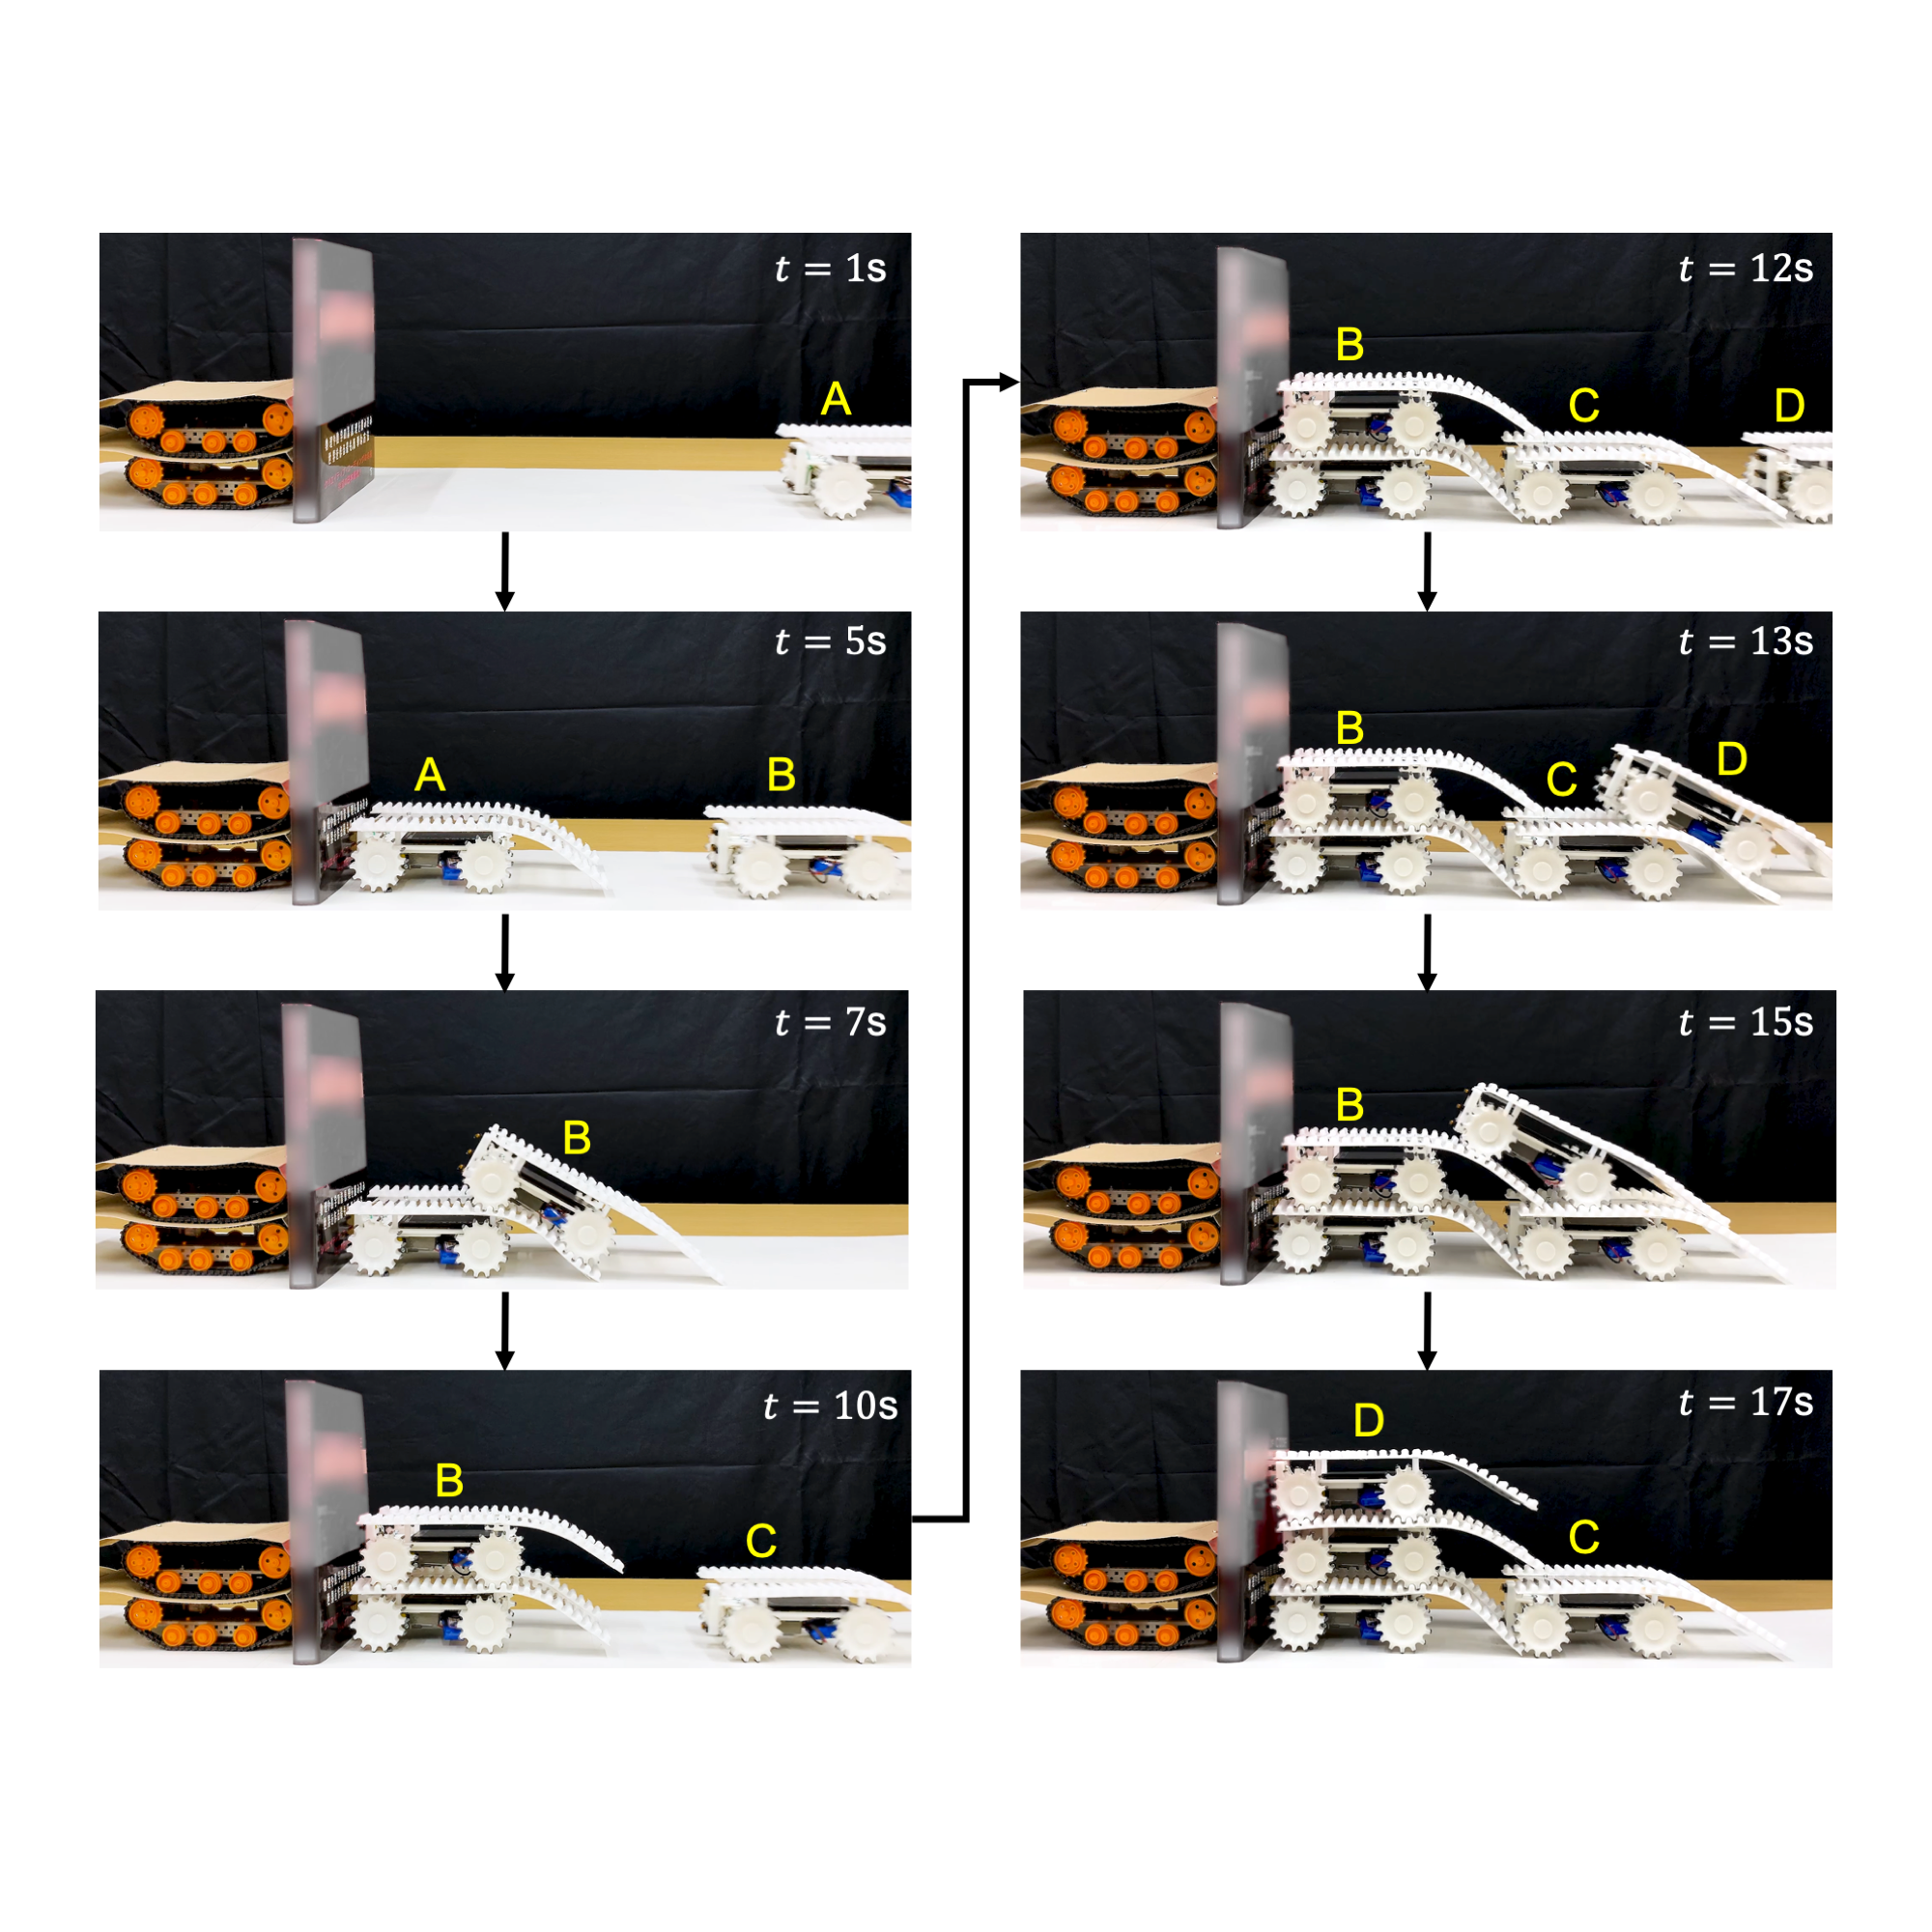
\includegraphics[width=\columnwidth]{figure/climb.pdf}
  \caption{Experiment of climbing over each other}
  \label{fig:climb}
\end{figure}

\subsection{考察}
このピニオン車輪とラックレール機構を使うと,ロボットが乗り上げる際に,ピニオン車輪は空転することや,滑ることがなく,安定に乗り上げられることが確認できた.また,一般に使われている車輪やクローラーより効率よく,安定に乗り上げることも言える.
そして,ロボットが乗り上げる際,前方のロボットを動かさずに乗り上げることができるので,前のロボットが物体を支持しているときでも,物体に影響を与えず,乗り上げられると言える.
その他,最初にピニオン車輪とラックレールがかみ合わなくても,車輪が回し続けると,自重で受動的にかみ合うことがわかった.よって,ロボットが1列縦隊であれば,どのような場合でもピニオン車輪をラックレールとかみ合わせられると言える.
%%%%%%%%%%%%%%%%%%%%%%%%%%%%%%%%%%%%%%%%%%%%%%%%%%%%%%%%%%%%%%%%%%%%%%%%%

\section*{牽引装置}
乗り上げることを確認できた後,物体の安定化性能に関する実験を行った.つまり,移動ロボットが移動しているとき,支持部のロボットが物体を支持できるかどうかを確認する.ここからの実験は提案システムの移動部をロボットの代わりとして,紙を使用した.また,紙を一定力で引っ張るために,\reffig{pulling-mechanism-concept}に示すような牽引装置を作製した.牽引装置はTAMIYA社のキャタピラ車をワイヤで机に前進しないように固定し,安定化電源で一定の電圧をかける.このとき,クローラーが摩擦よって,紙を巻き取り,紙の上に載せているものを一定速度で動かすことができる.また,\reffig{pulling-mechanism}に示すように,クローラーと紙の間の摩擦を上げるために,グリップ力の高いの脱着式の軟質樹脂製パッドのついている連結式クローラーを利用した.そして,接触面積を大きくするために,クローラーをひっくり返し,さらにクローラーと紙の間の摩擦を大きくするために,クローラー車の上に巻きはんだを載せておもりとして利用した.
\begin{figure}[b]
  \centering
  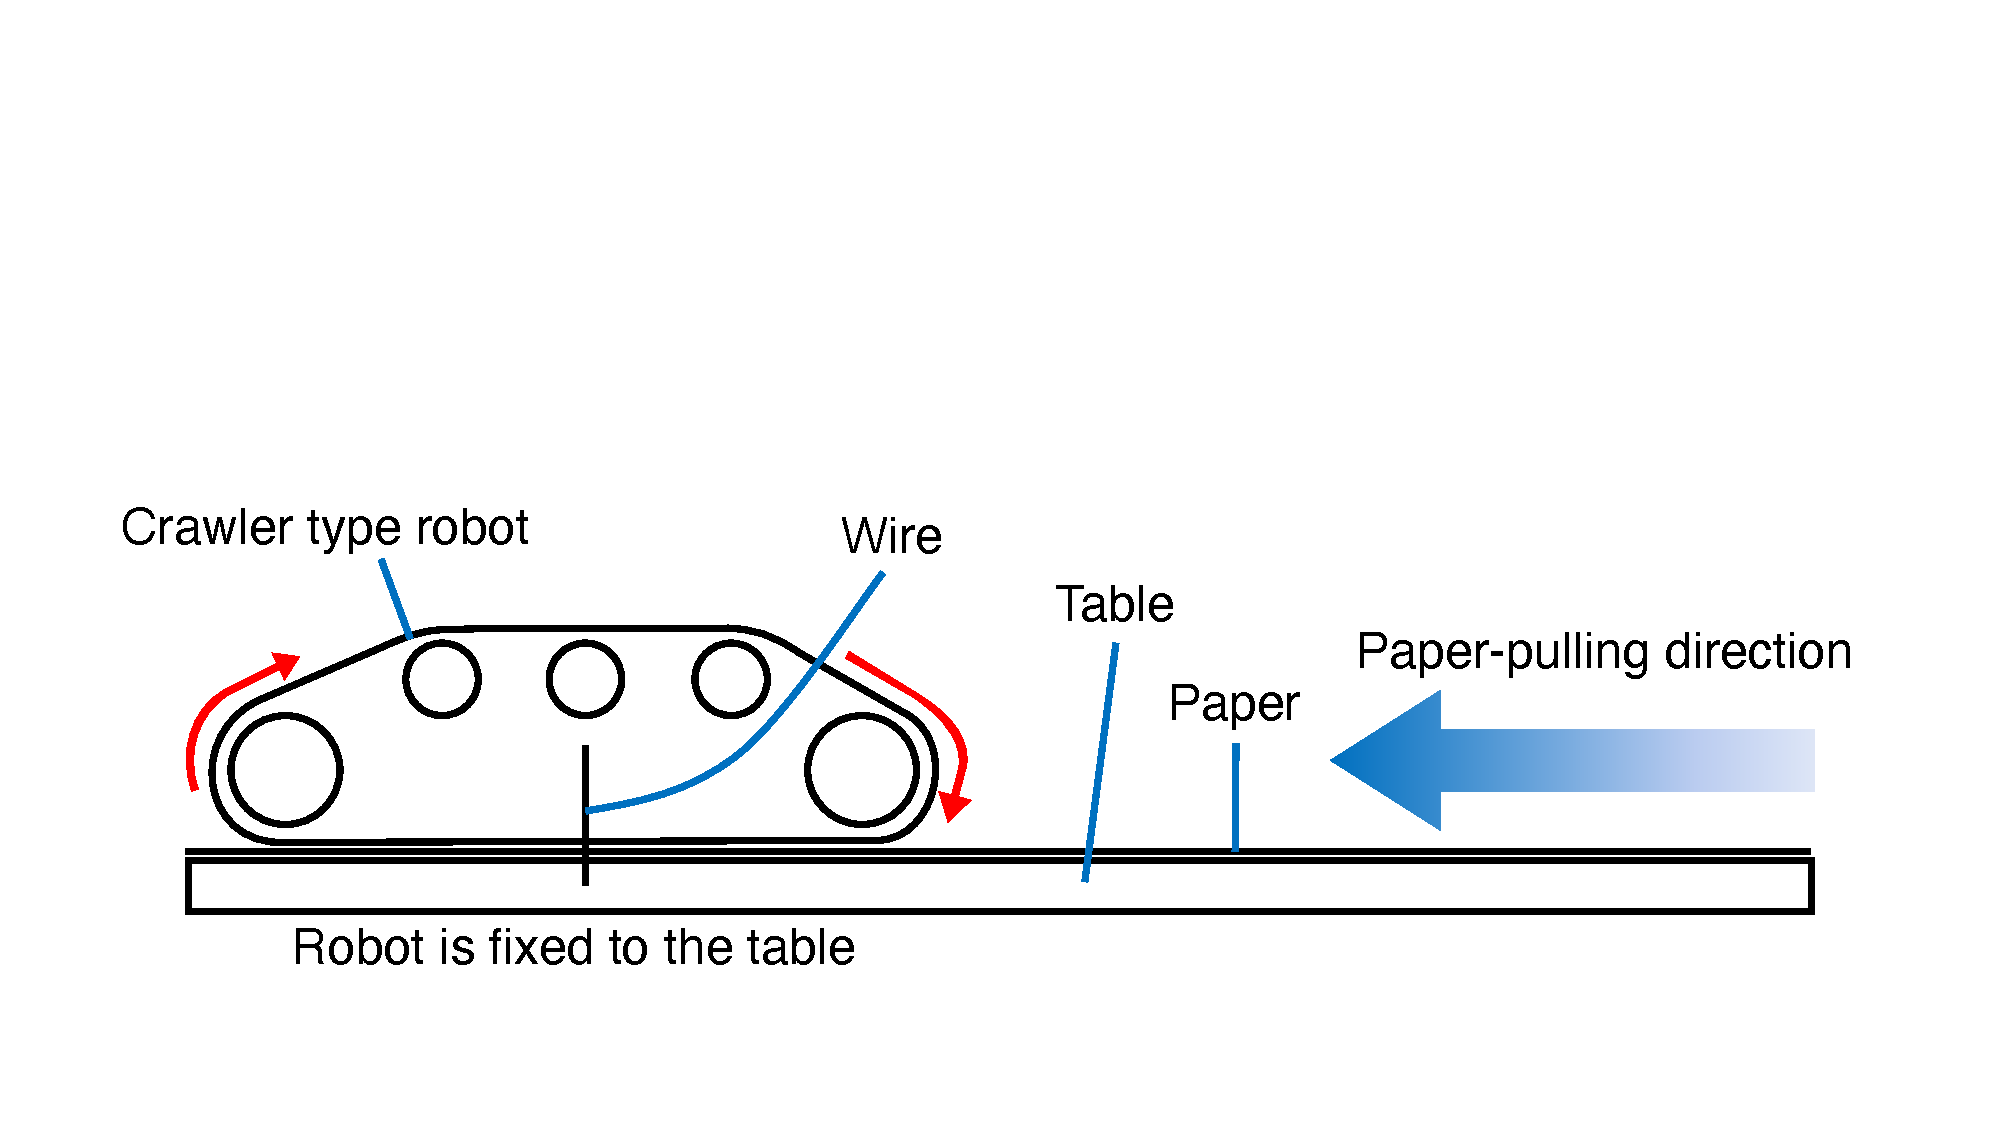
\includegraphics[width=0.75\columnwidth]{figure/concept-pulling-mechanism.pdf}
  \caption{Concept of pulling mechanism}
  \label{fig:pulling-mechanism-concept}
\end{figure}
\begin{figure}[tb]
  \centering
  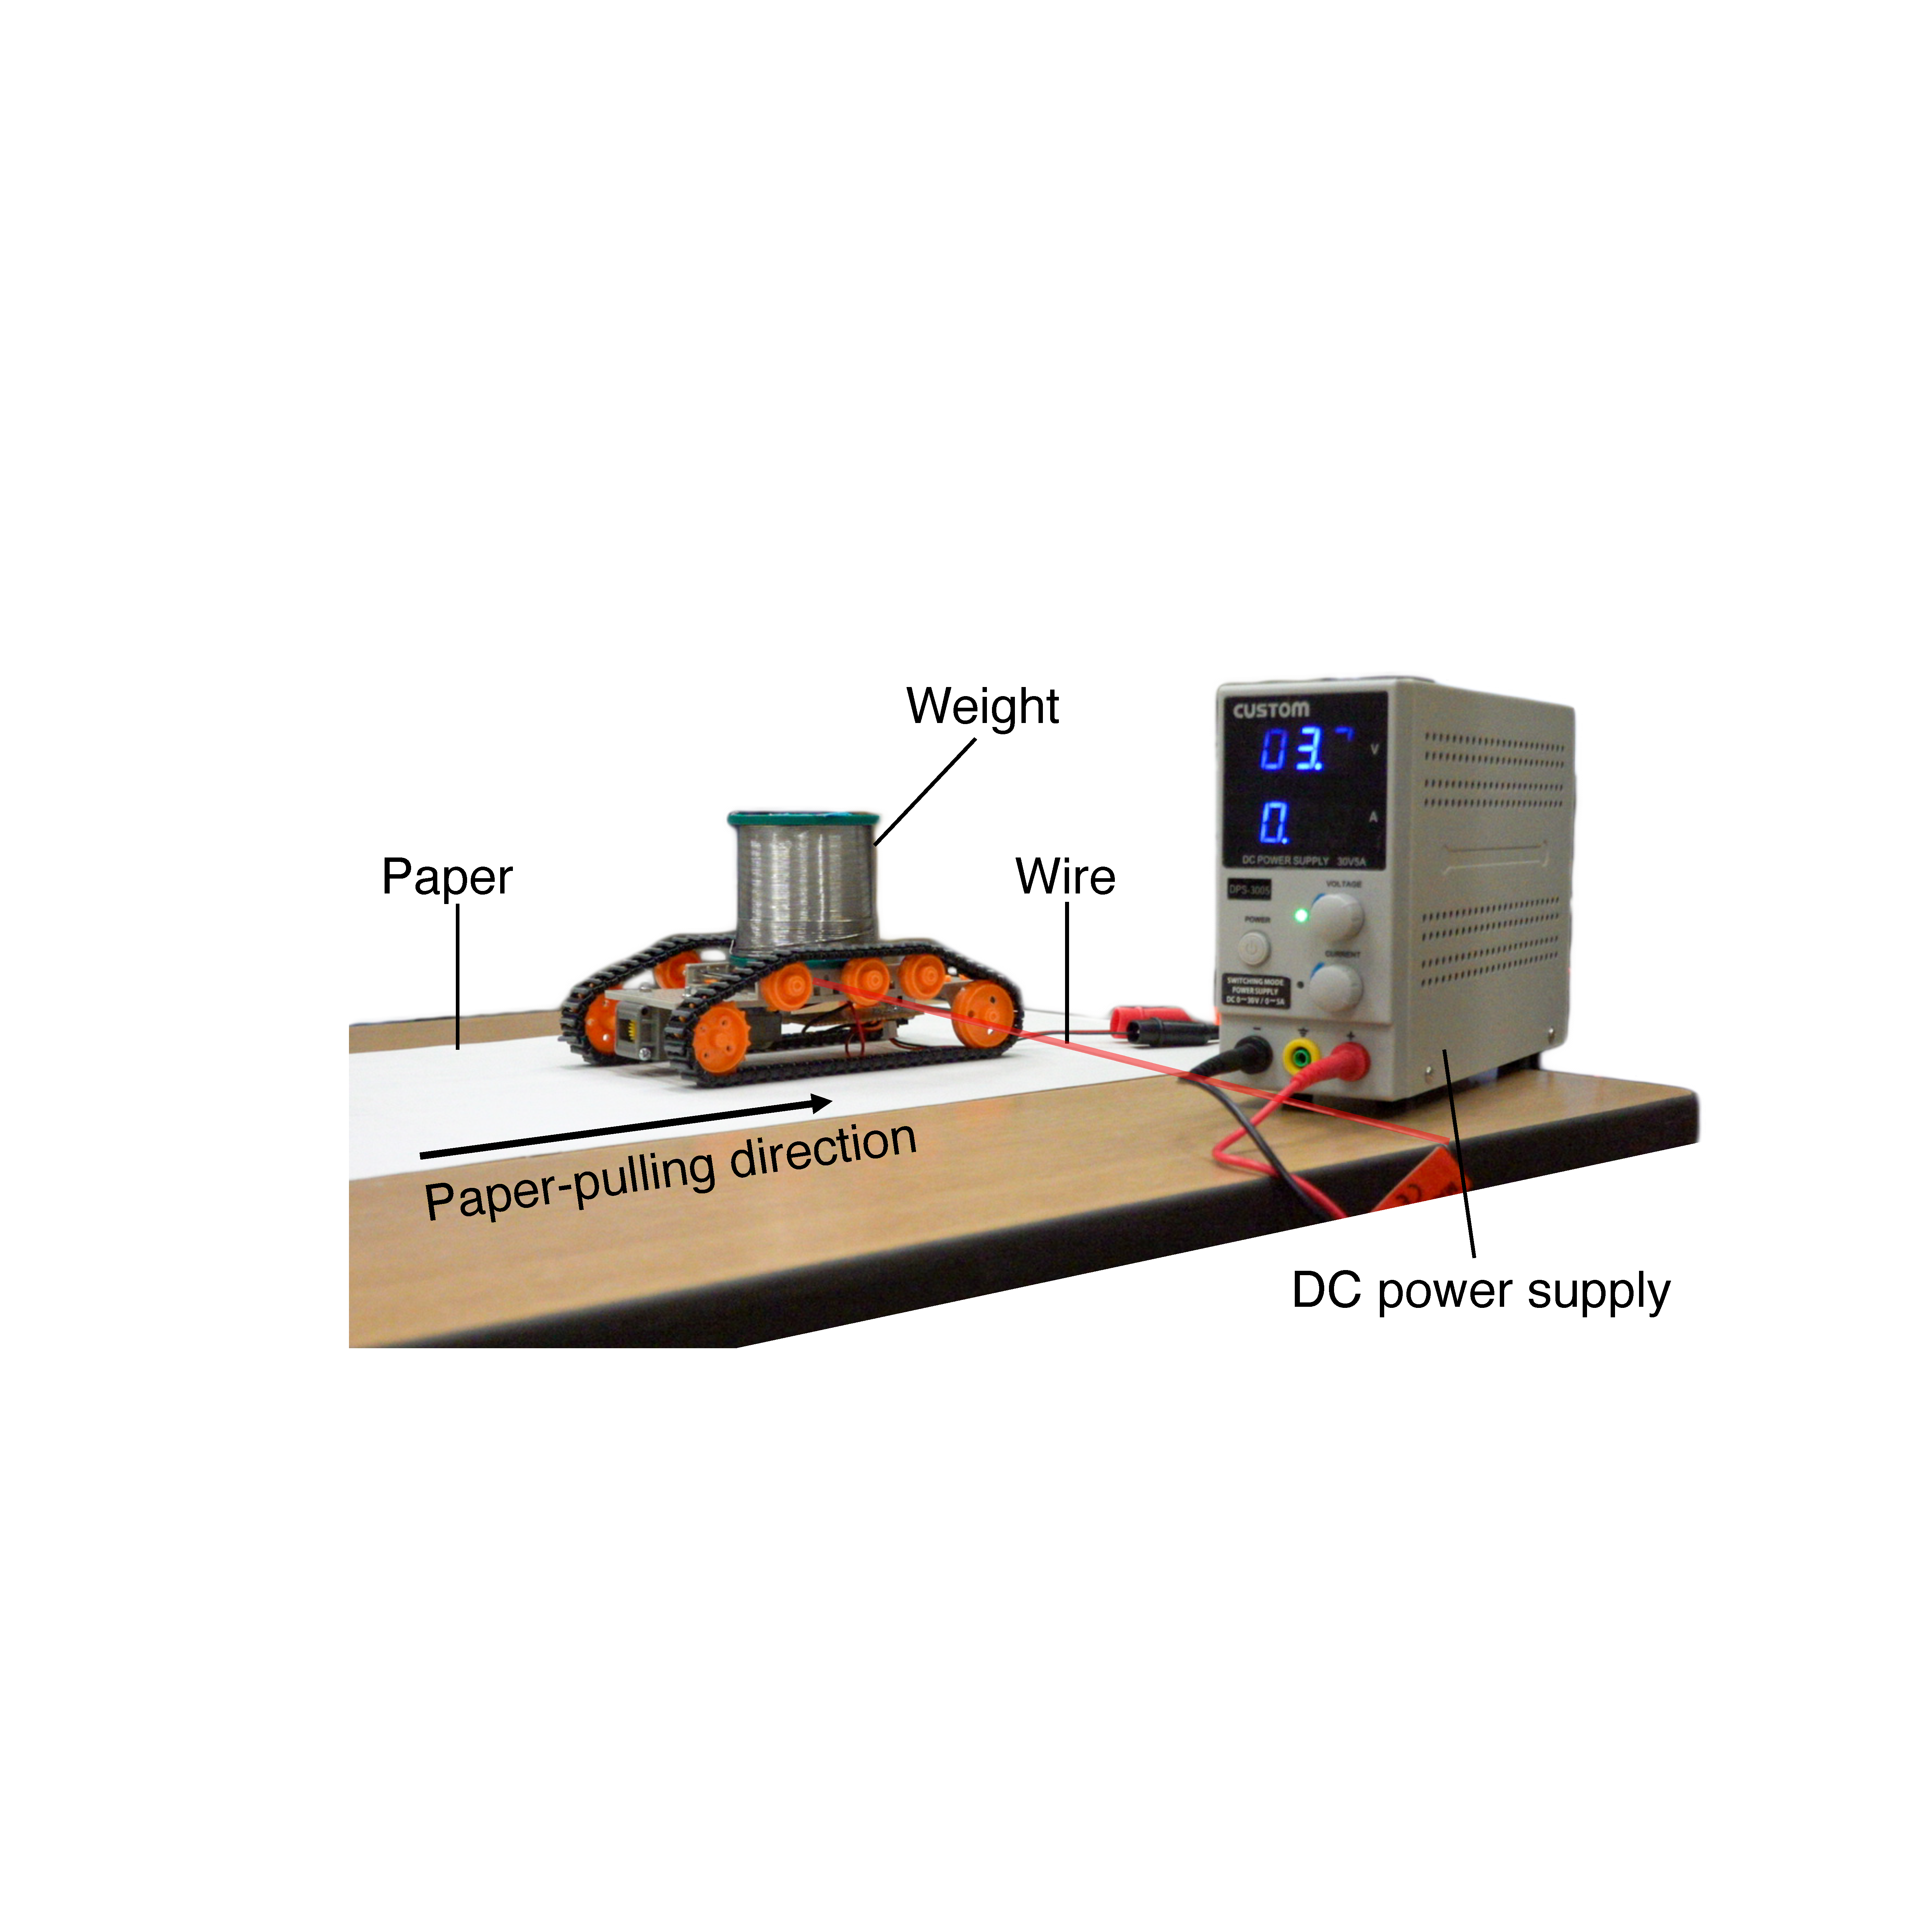
\includegraphics[width=0.7\columnwidth]{figure/pulling-mechanism-v2.pdf}
  \caption{Pulling mechanism}
  \label{fig:pulling-mechanism}
\end{figure}

また,物体の姿勢を評価するために,\reffig{gopro}に示すように,紙の上にカメラ(GoPro Hero 3 Black)を固定した.これによってカメラを搬送物体と同じ速度で動かすことができ,トラッキングによって物体の角度を計測することが可能である.

\begin{figure}[tb]
  \centering
  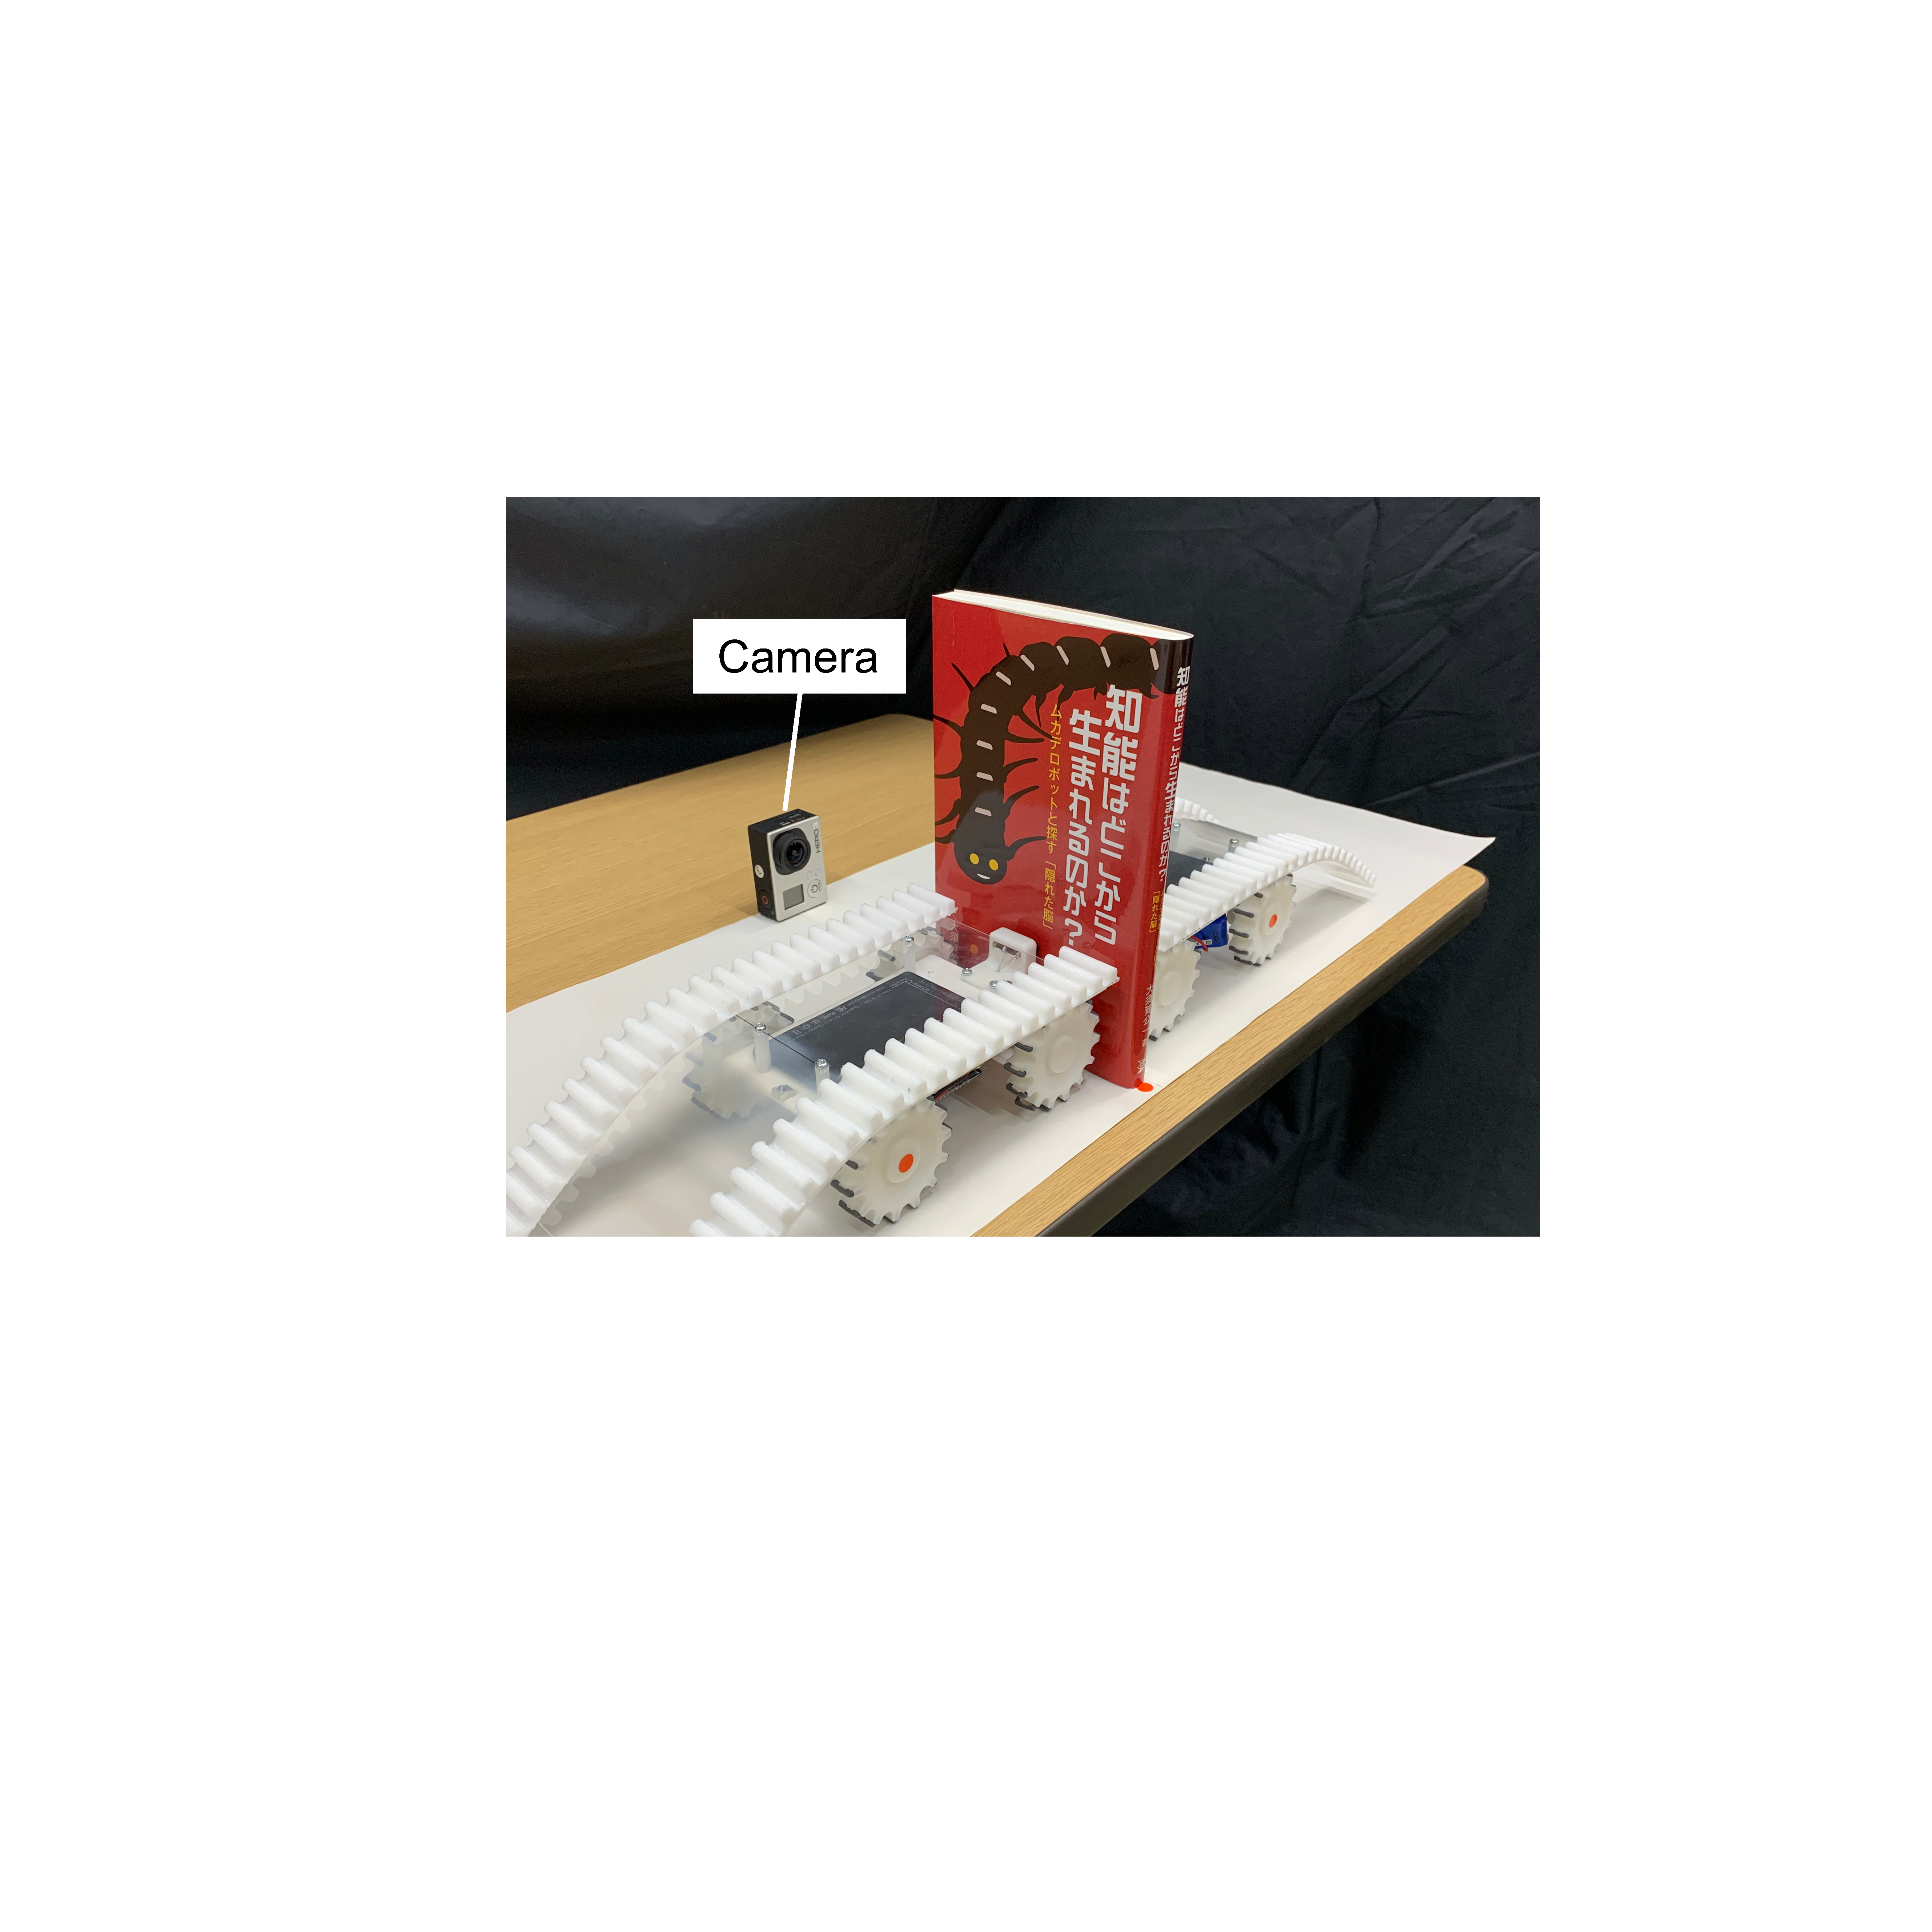
\includegraphics[width=0.7\columnwidth]{figure/gopro.pdf}
  \caption{Camera for tracking the angle of object}
  \label{fig:gopro}
\end{figure}
この牽引装置を利用して,以下の実験を行った.

\section{段数の変更による物体の安定化性能に関する実験}
\label{section:exp2}
~\ref{section:modeling}で述べたロボットと物体の高さの比$\frac{h_{r}}{h_{o}}$を大きくすることにより物体をより安定に支持することを検証するために,
製作したロボットを積み重ねることで,物体を支持することが可能であるかの検証を行った.さらに全体の加速度と物体の角度の解析を行った.

\subsection{実験手順}
上で述べた紙の上に,搬送物体として本を立てて置いた.その両側にロボットを1段ずつと2段ずつ置き,牽引装置に6Vの電圧を印加したときの安定化性能の比較を行った.

\subsection{実験結果と考察}
まず,物体の両側にロボットを1段および2段置いた場合の実験の様子を\reffig{exp-layers}に示す.また,そのときの全体の加速度の変化と物体の角度の変化を\reffig{acc-1v2}と\reffig{angle-1v2}にそれぞれ示す.
\begin{figure}[tb]
  \vspace{0mm}
  \centering
  \begin{tabular}{c}
    \begin{minipage}[ht]{0.5\columnwidth}
      \centering
      \includegraphics[width=\columnwidth]{figure/1layer.pdf}
      \subcaption{1 layer}
      \labfig{6v-1layer}
    \end{minipage}
    \begin{minipage}[ht]{0.5\columnwidth}
      \centering
      \includegraphics[width=\columnwidth]{figure/2layers.pdf}
      \subcaption{2 layers}
      \labfig{6v-2layer}
    \end{minipage}
  \end{tabular}
  \centering
  \caption{Experiment of changing supporting layers}
  \labfig{exp-layers}
\end{figure}

\reffig{6v-1layer}より,ロボットが1段の場合では紙を引っ張り出すと,物体はすぐ倒れた.一方,\reffig{6v-2layer}より,ロボットが2段の場合では紙を引っ張り出してから止まるまで物体は最初の姿勢を保つことができた.
\begin{figure}[tb]
 \centering
  \begin{tabular}{c}
   
   \begin{minipage}{\hsize}
    \centering
     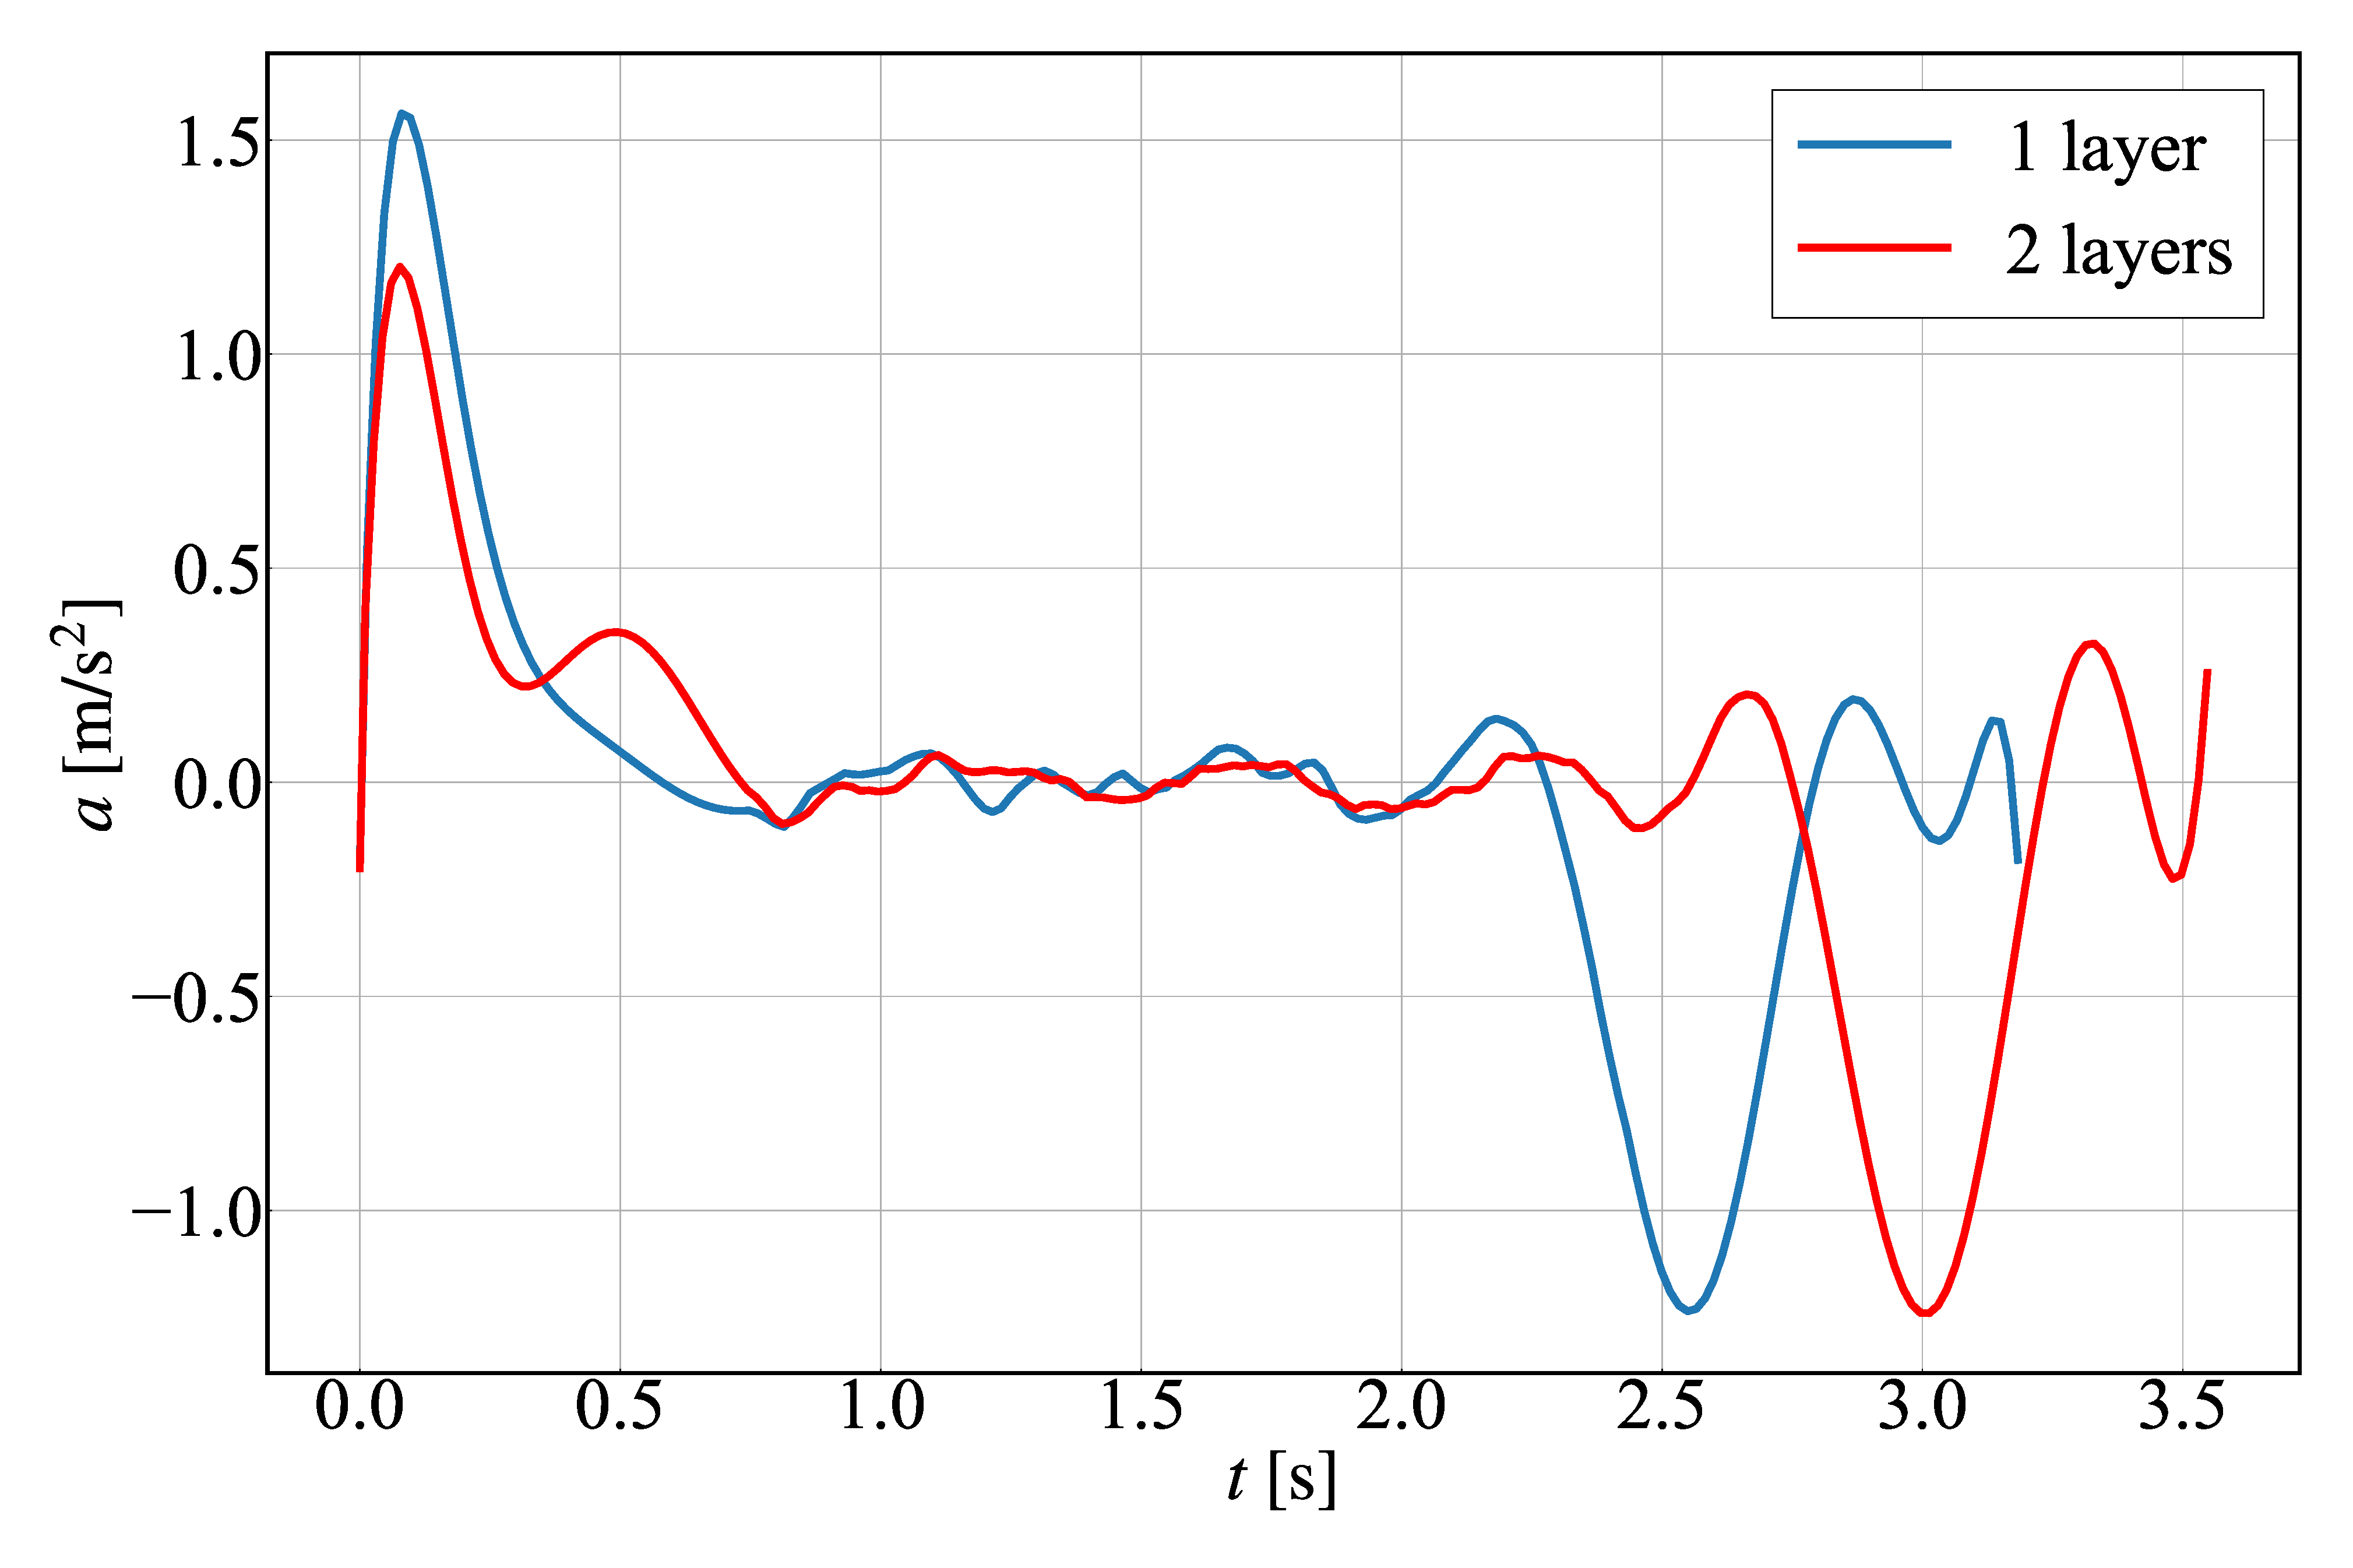
\includegraphics[width=0.63\columnwidth, angle=0]{figure/acc-graph-1v2.eps}
     \caption{Change in acceleration (Layer)}
     \labfig{acc-1v2}
   \end{minipage}\\
   
   \begin{minipage}{\hsize}
    \centering
     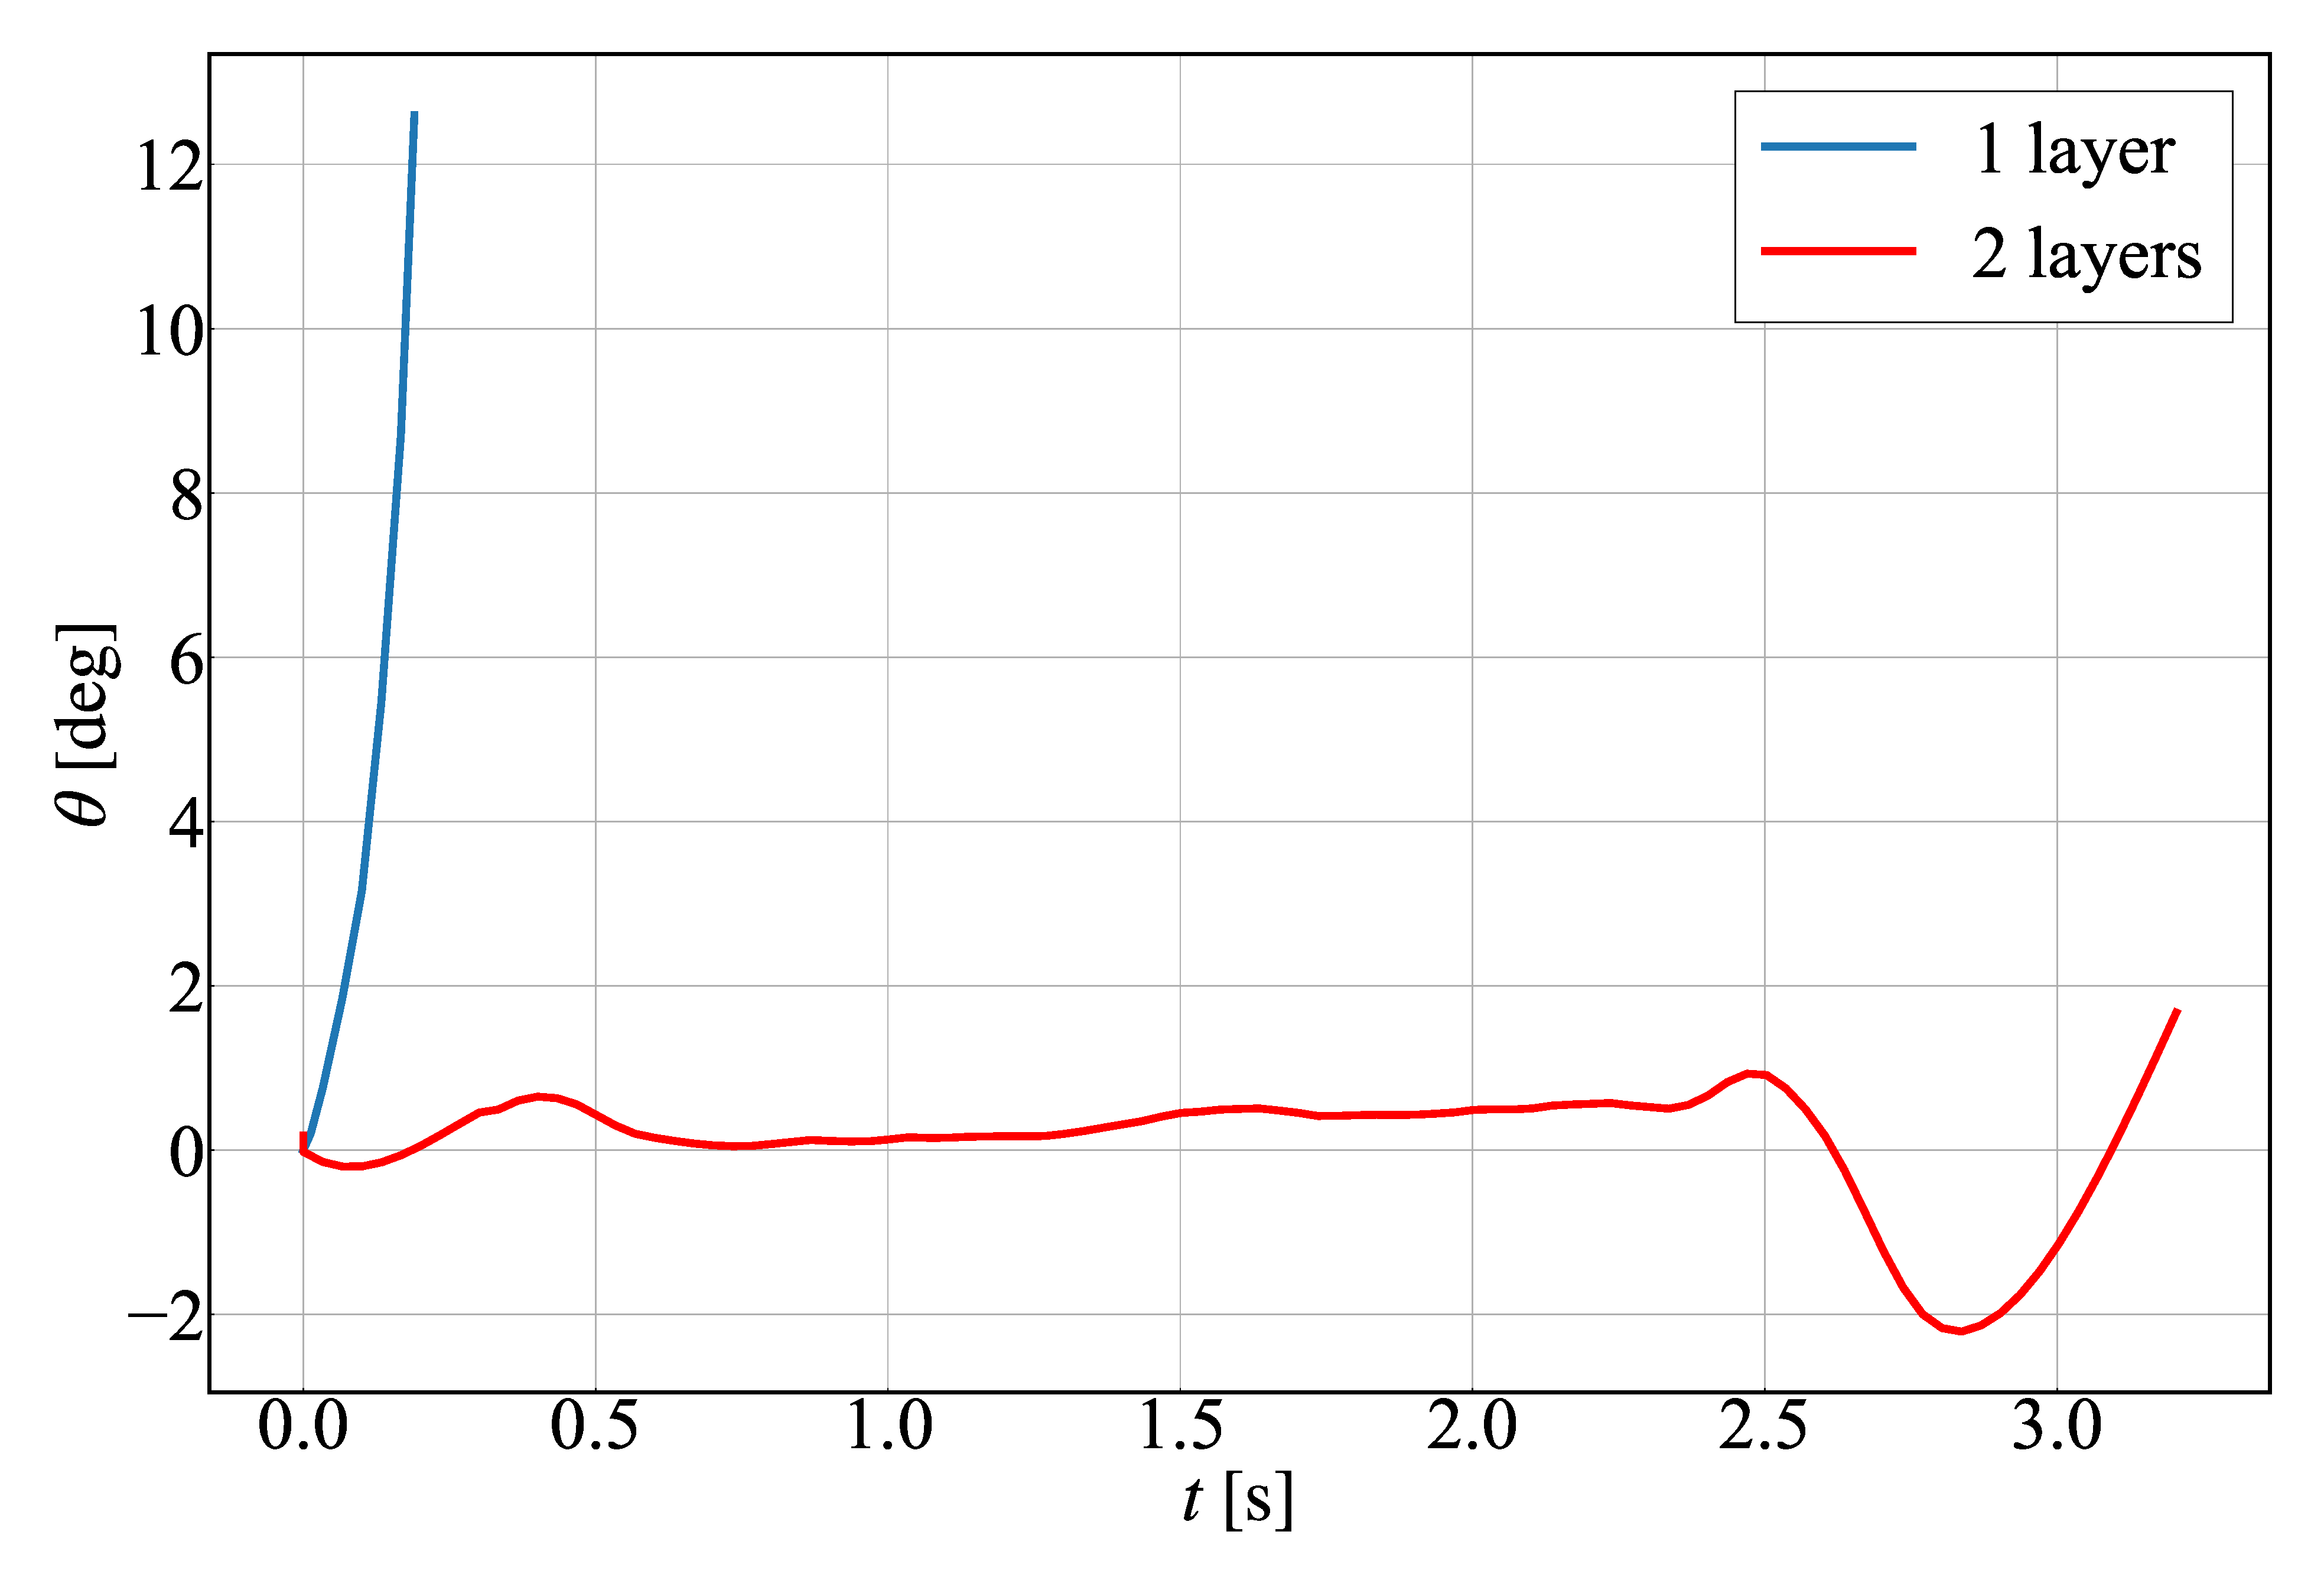
\includegraphics[width=0.6\columnwidth, angle=0]{figure/angle-1vs2.eps}
     \caption{Change in angle (Layer)}
     \labfig{angle-1v2}
   \end{minipage}
  \end{tabular}
\end{figure}

そして,\reffig{acc-1v2}では,横軸は時間,縦軸は紙の動く加速度である.\reffig{acc-1v2}より,牽引装置に電圧を印加する瞬間,つまり時刻が$t=0$~sから$t=0.5$~sの間では1段と2段の場合とも加速されていることがわかった.そのとき,1段の場合の全体の最大加速度は$a_{max}=1.5$~\si{m/s^2}であったが,2段の場合は$a_{max}=1.3$~\si{m/s^2}であった.その原因は2段に積むと,支持部全体の質量は1段の方より大きいので,紙と机の間の摩擦は1段より大きいと考えられる.
$t=0.5$~sから$t=2.3$~sの間では加速度は0~\si{m/s^2}付近であり,等速で移動することが確認できた.その後,牽引装置の印加電圧を遮断すると,全体が減速し,止まった.
次に,\reffig{angle-1v2}では,横軸は時間,縦軸は物体の初期姿勢からの角度のずれである.ここで,物体の角度は進行方向の逆向きを正とする.1段の場合の角度は設定された$\pm5$\si{\degree}範囲外にあることがわかった.一方2段の場合は動き出してから,減速までの間で$-0.3$\si{\degree}$\sim0.9$\si{\degree}に収まることが確認できた.
この結果より,牽引装置の印加電圧が6Vのとき,全体の加速度が大きいため,1段で支持する場合はロボットが滑ってしまい,物体を支持できなくなる.しかし,2段に増やすと,物体の重心近くで支持することと,2段のロボットが紙から滑りにくくなることによって,物体を支持し,移動することができると考えられる.

\section{制御による物体の安定化性能に関する実験}
\label{section:exp3}
~\ref{section:modeling}で述べたロボット1とロボット2の前進力$F_{r_{1}}$,$F_{r_{2}}$を加えることにより物体をより安定に支持することを検証するために,
製作したロボットの物体の姿勢を検知するセンサを利用し,物体の初期姿勢に戻そうとする制御をかけると,前節では物体を支持することができなかったロボットが1段の場合でも,物体を支持できるかを確認する実験を行った.さらに全体の加速度と物体の角度の解析を行った.

\subsection{実験手順}
まず,かける制御について述べる.それを\reffig{overview-control}に示す.\reffig{upright}より,物体の姿勢を検知するセンサの上下両方のスイッチが反応したとき,ロボットに対して物体は安定であると判断し,ロボットは前進しない.
しかし,\reffig{tilt}より,もし物体が右に傾いている場合,左のロボットに取り付けられた物体の姿勢を検知するセンサは下のスイッチのみ反応するが,一方,右のロボットに取り付けられたセンサは上のスイッチのみ反応する.このとき,右のロボットが左のロボットより大きい速度で物体を押し付けることで,物体の姿勢を保つと考える.
\begin{figure}[tb]
 \centering
  \begin{tabular}{c}
   
   \begin{minipage}{\hsize}
    \centering
    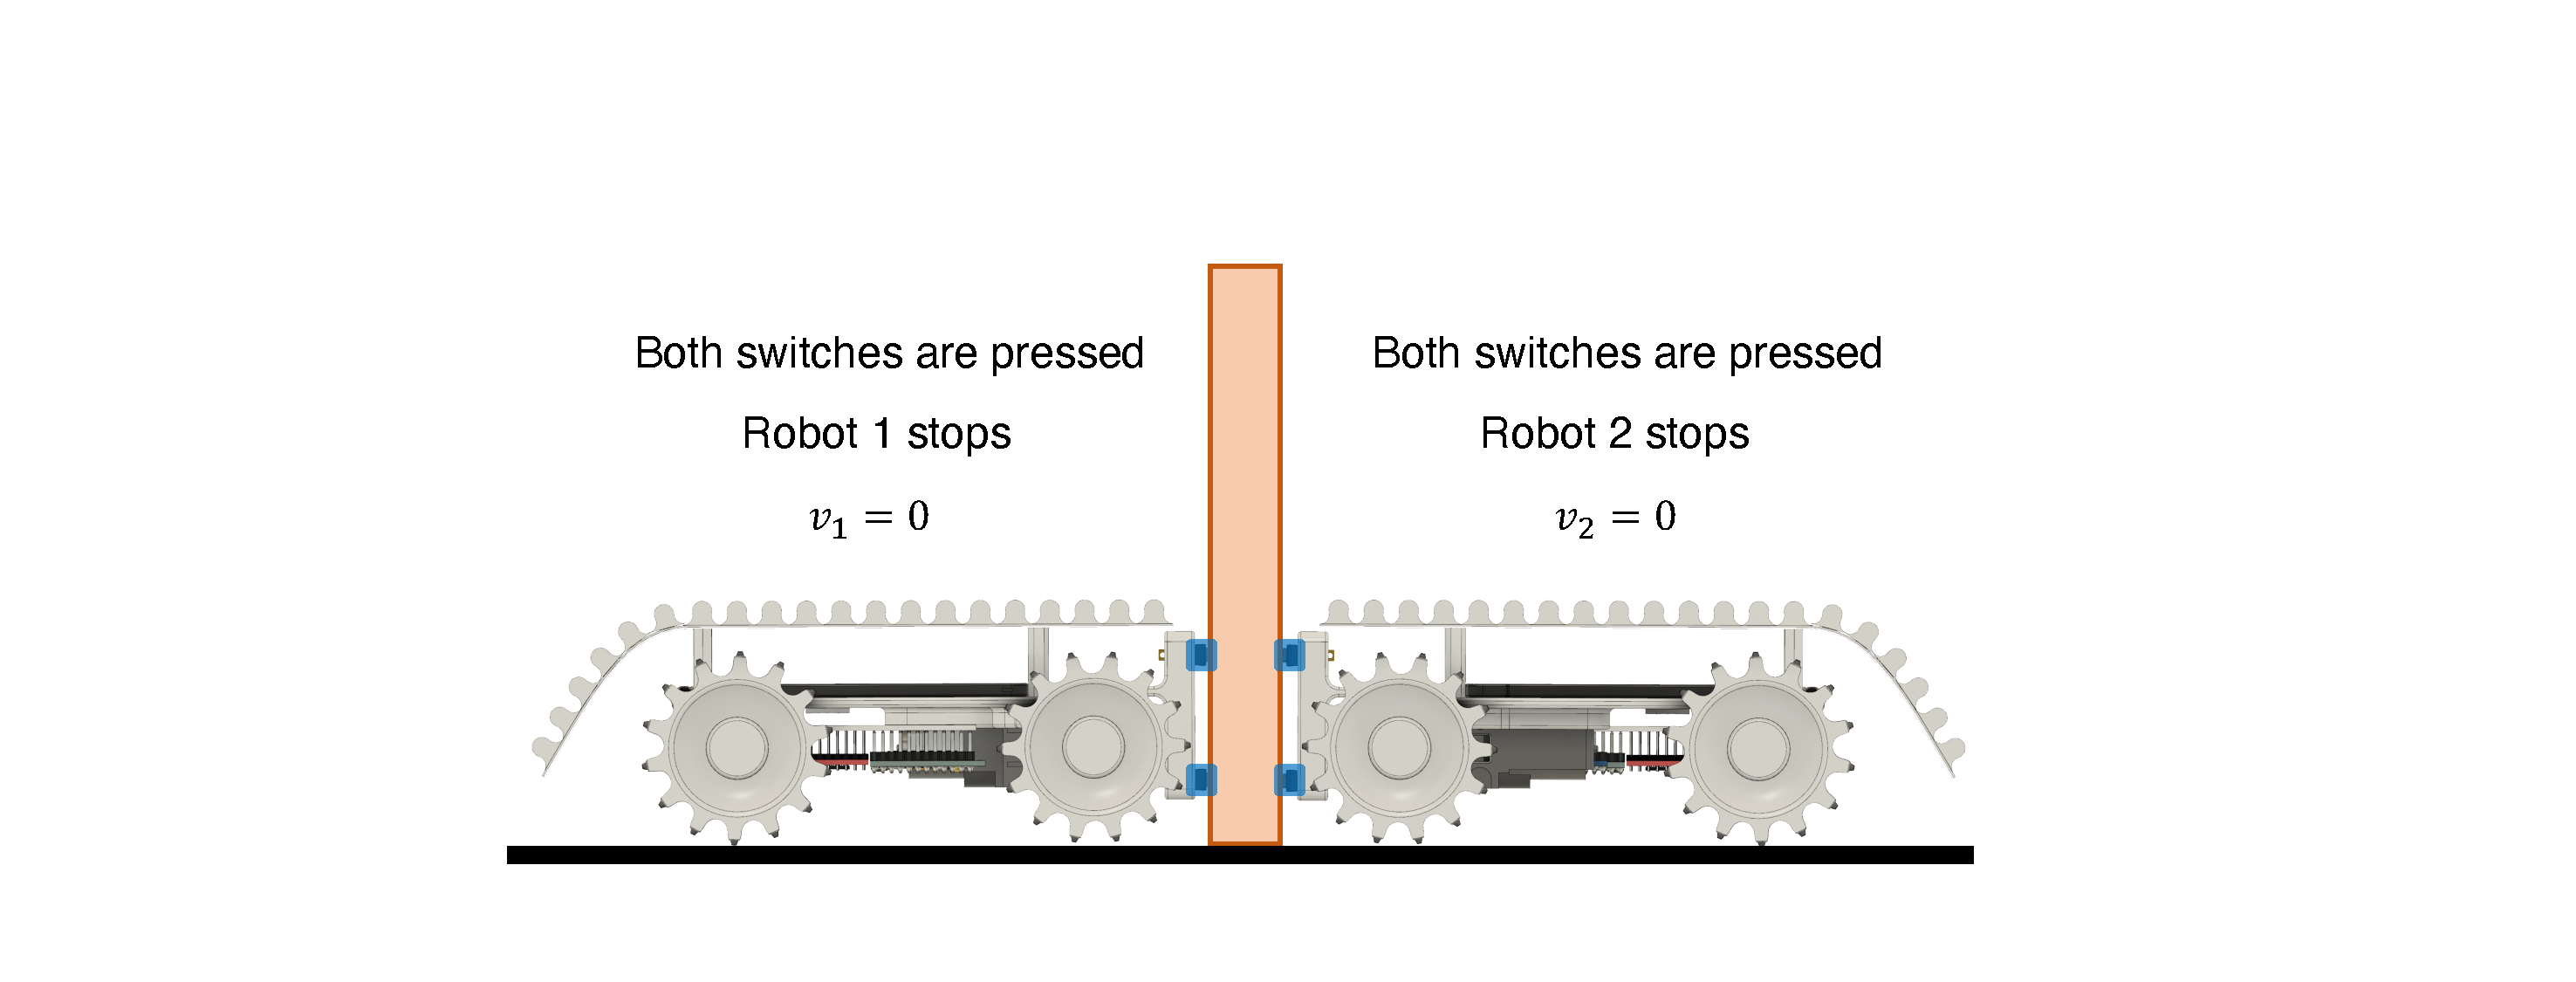
\includegraphics[width=0.8\columnwidth]{figure/control-upright.pdf}
      \subcaption{Object is upright}
      \label{fig:upright}
   \end{minipage}\\
   
   \begin{minipage}{\hsize}
    \centering
    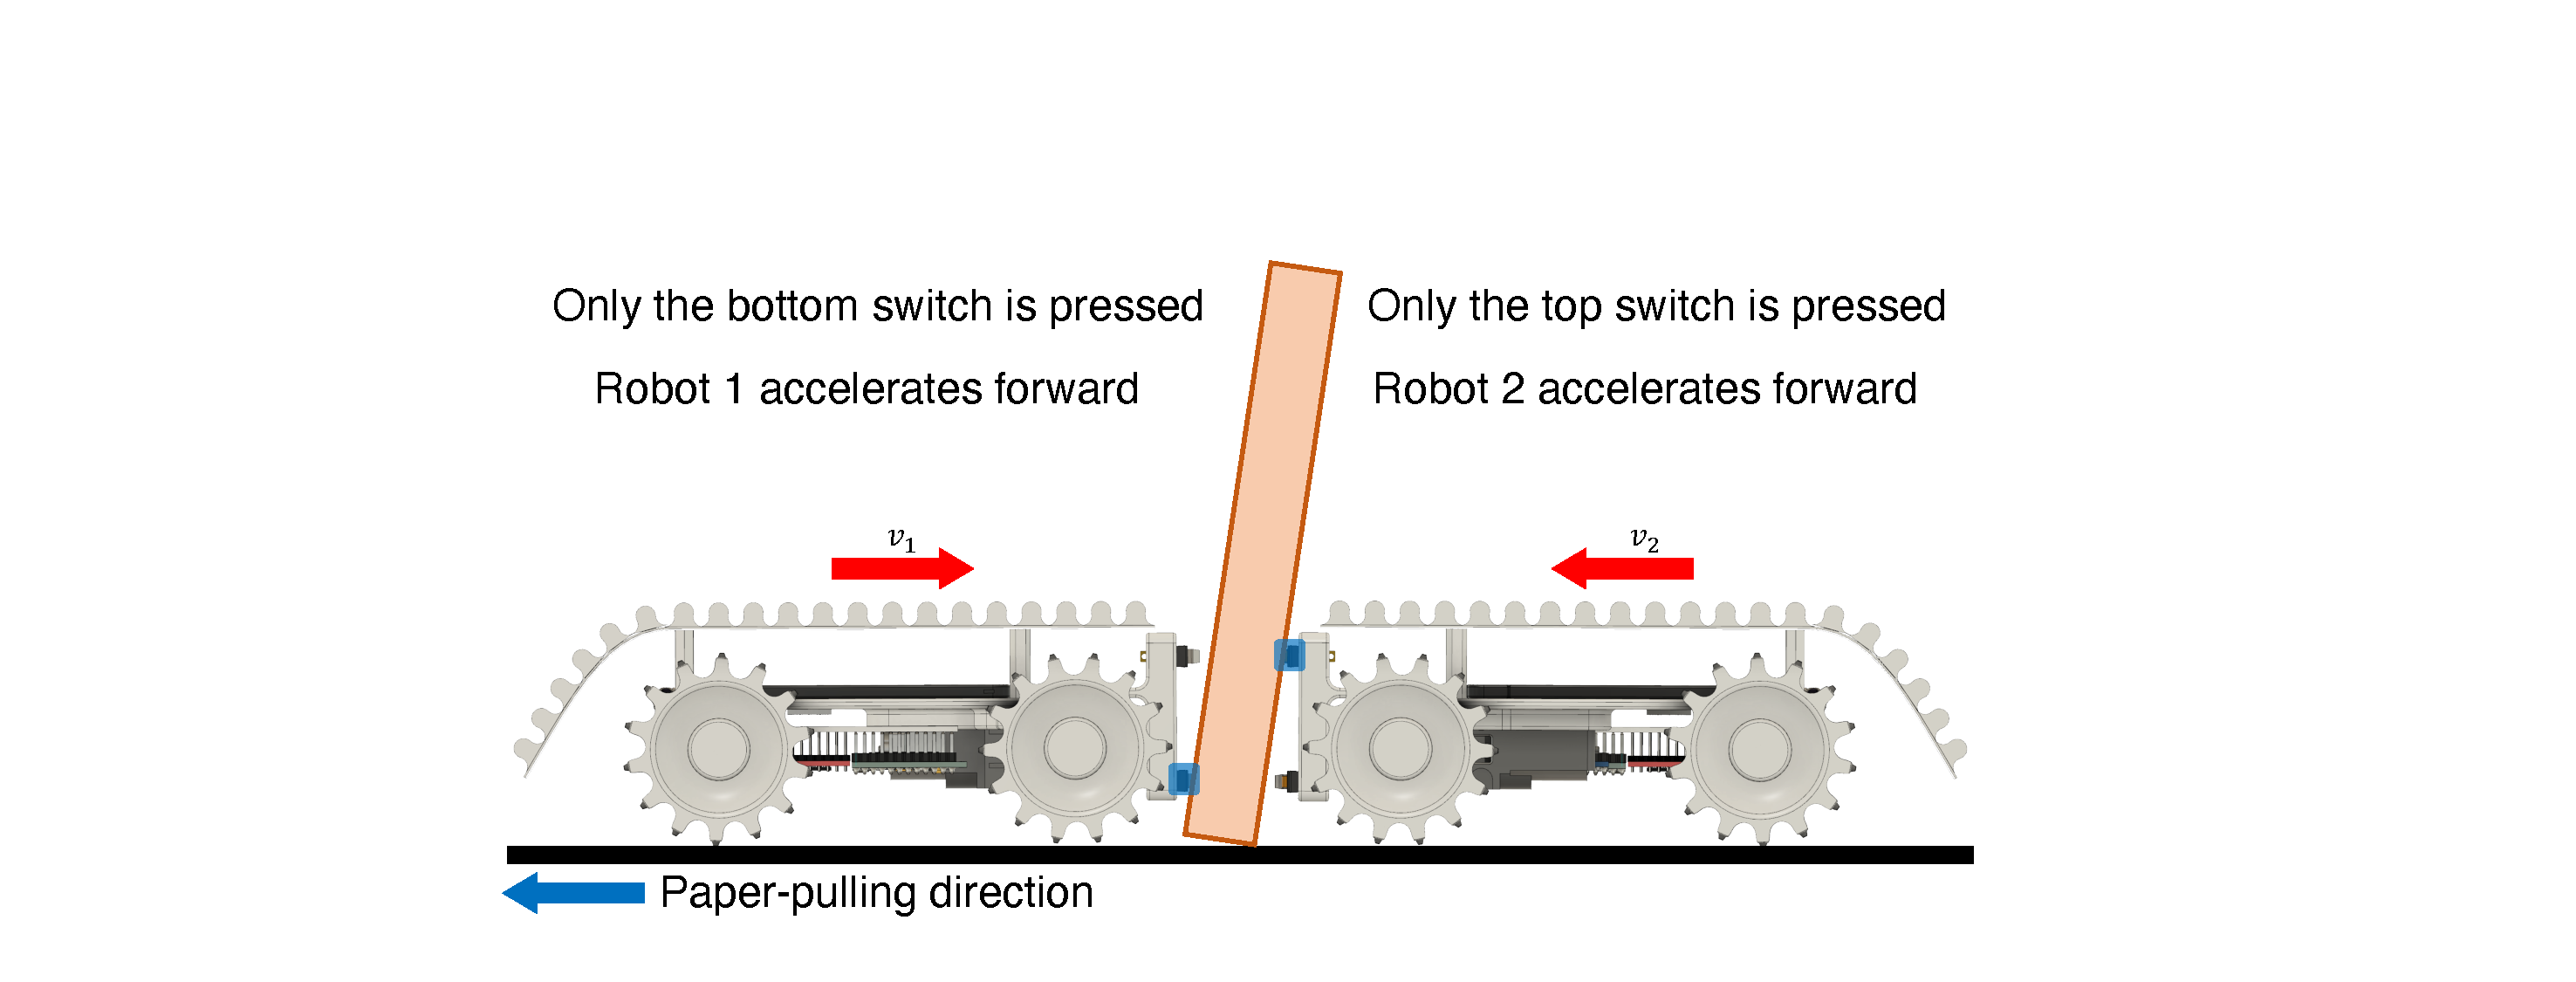
\includegraphics[width=0.8\columnwidth]{figure/control-tilted-v2.pdf}
      \subcaption{Object is tilted}
      \label{fig:tilt}
   \end{minipage}
  \end{tabular}
  \caption{Overview of control system}
  \label{fig:overview-control}
\end{figure}

~\ref{section:exp2}で述べた実験と同じく,ロボットを物体の両側に置いて,牽引装置に6Vの電圧を印加した場合について,安定化性能の比較を行った.

\subsection{実験結果と考察}
まず,物体の姿勢を検知するセンサによって制御をかけた場合の実験の様子を\reffig{control}に示す.また,そのときの全体の加速度の変化と物体の角度の変化を\reffig{acc-1vC}と\reffig{angle-1vC}にそれぞれを示す.
\begin{figure}[tb]
  \centering
  \includegraphics[width=0.6\columnwidth]{figure/control.pdf}
  \caption{Experiment of applying control}
  \label{fig:control}
\end{figure}

\reffig{control}より,紙を引っ張り出した瞬間,ロボットはまだ反応していないときに,物体は傾いた.しかし,その後はロボットのセンサが反応するため,ロボットが物体を初期姿勢に戻そうとする.これによって全体が止まるまで物体を支持できることが確認できた.

\begin{figure}[tb]
 \centering
  \begin{tabular}{c}
   
   \begin{minipage}{\hsize}
    \centering
     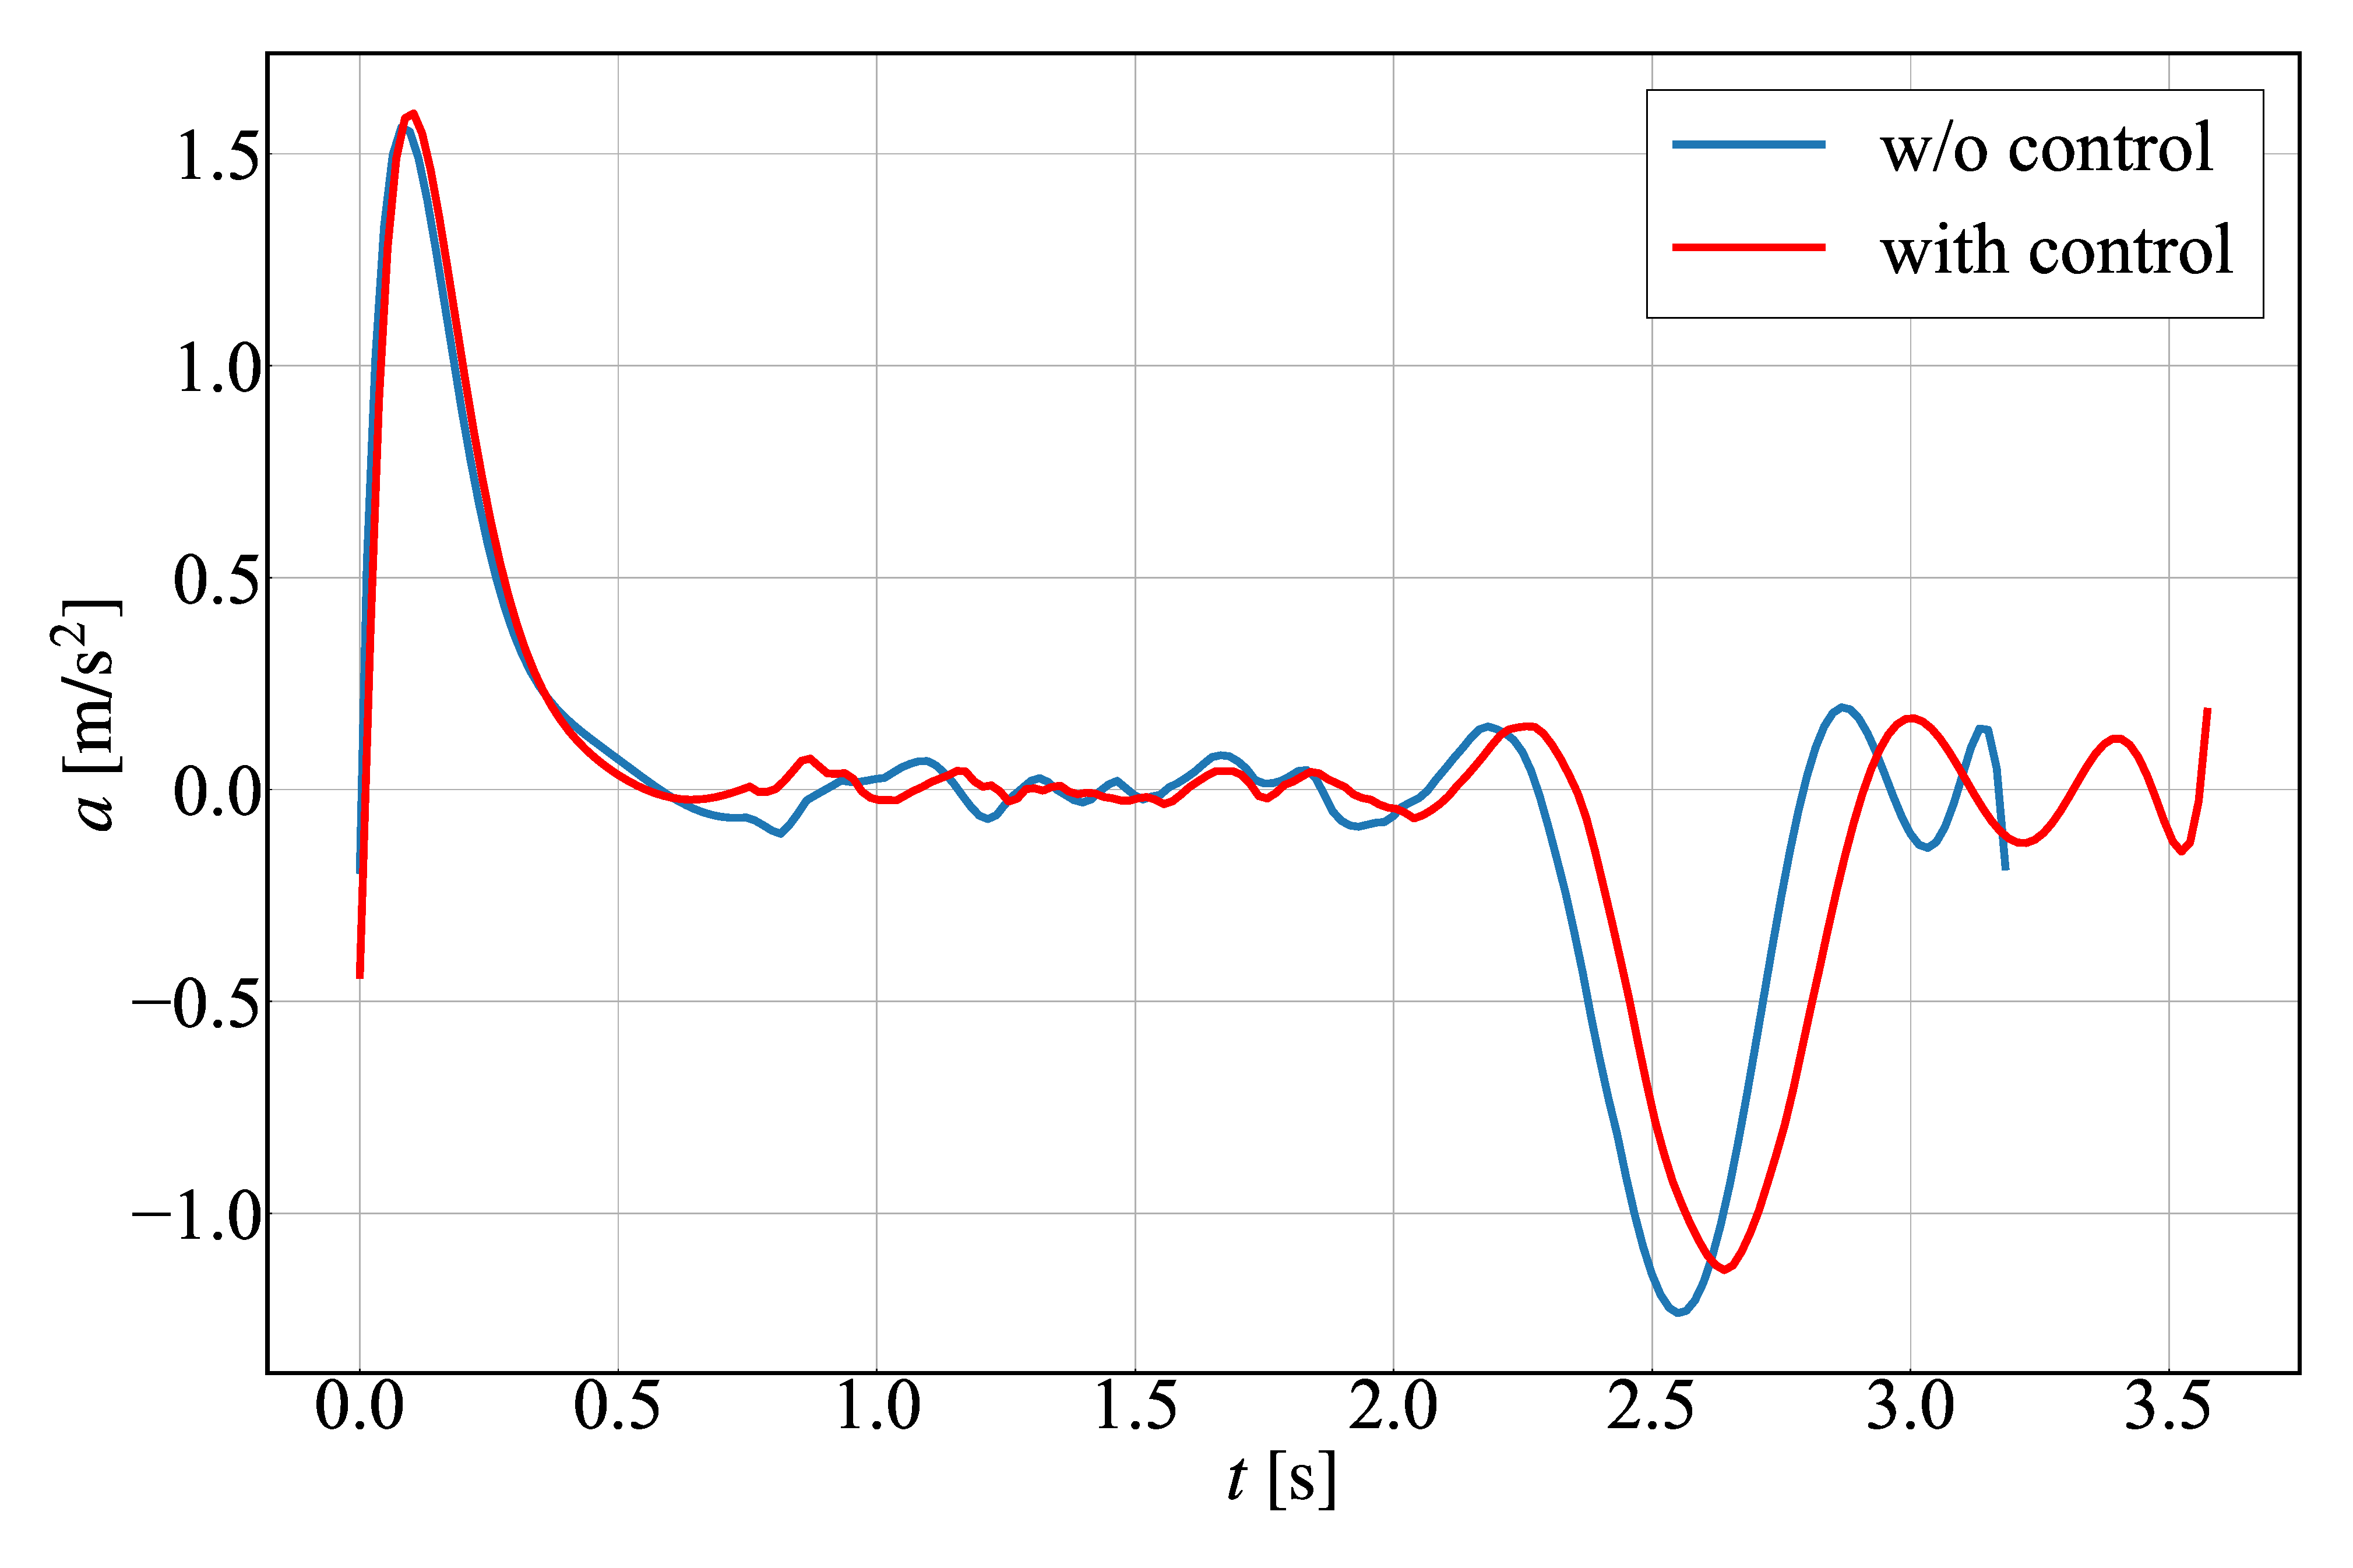
\includegraphics[width=0.63\columnwidth]{figure/acc-graph-control.eps}
     \caption{Change in acceleration (Control)}
     \labfig{acc-1vC}
   \end{minipage}\\
   
   \begin{minipage}{\hsize}
    \centering
     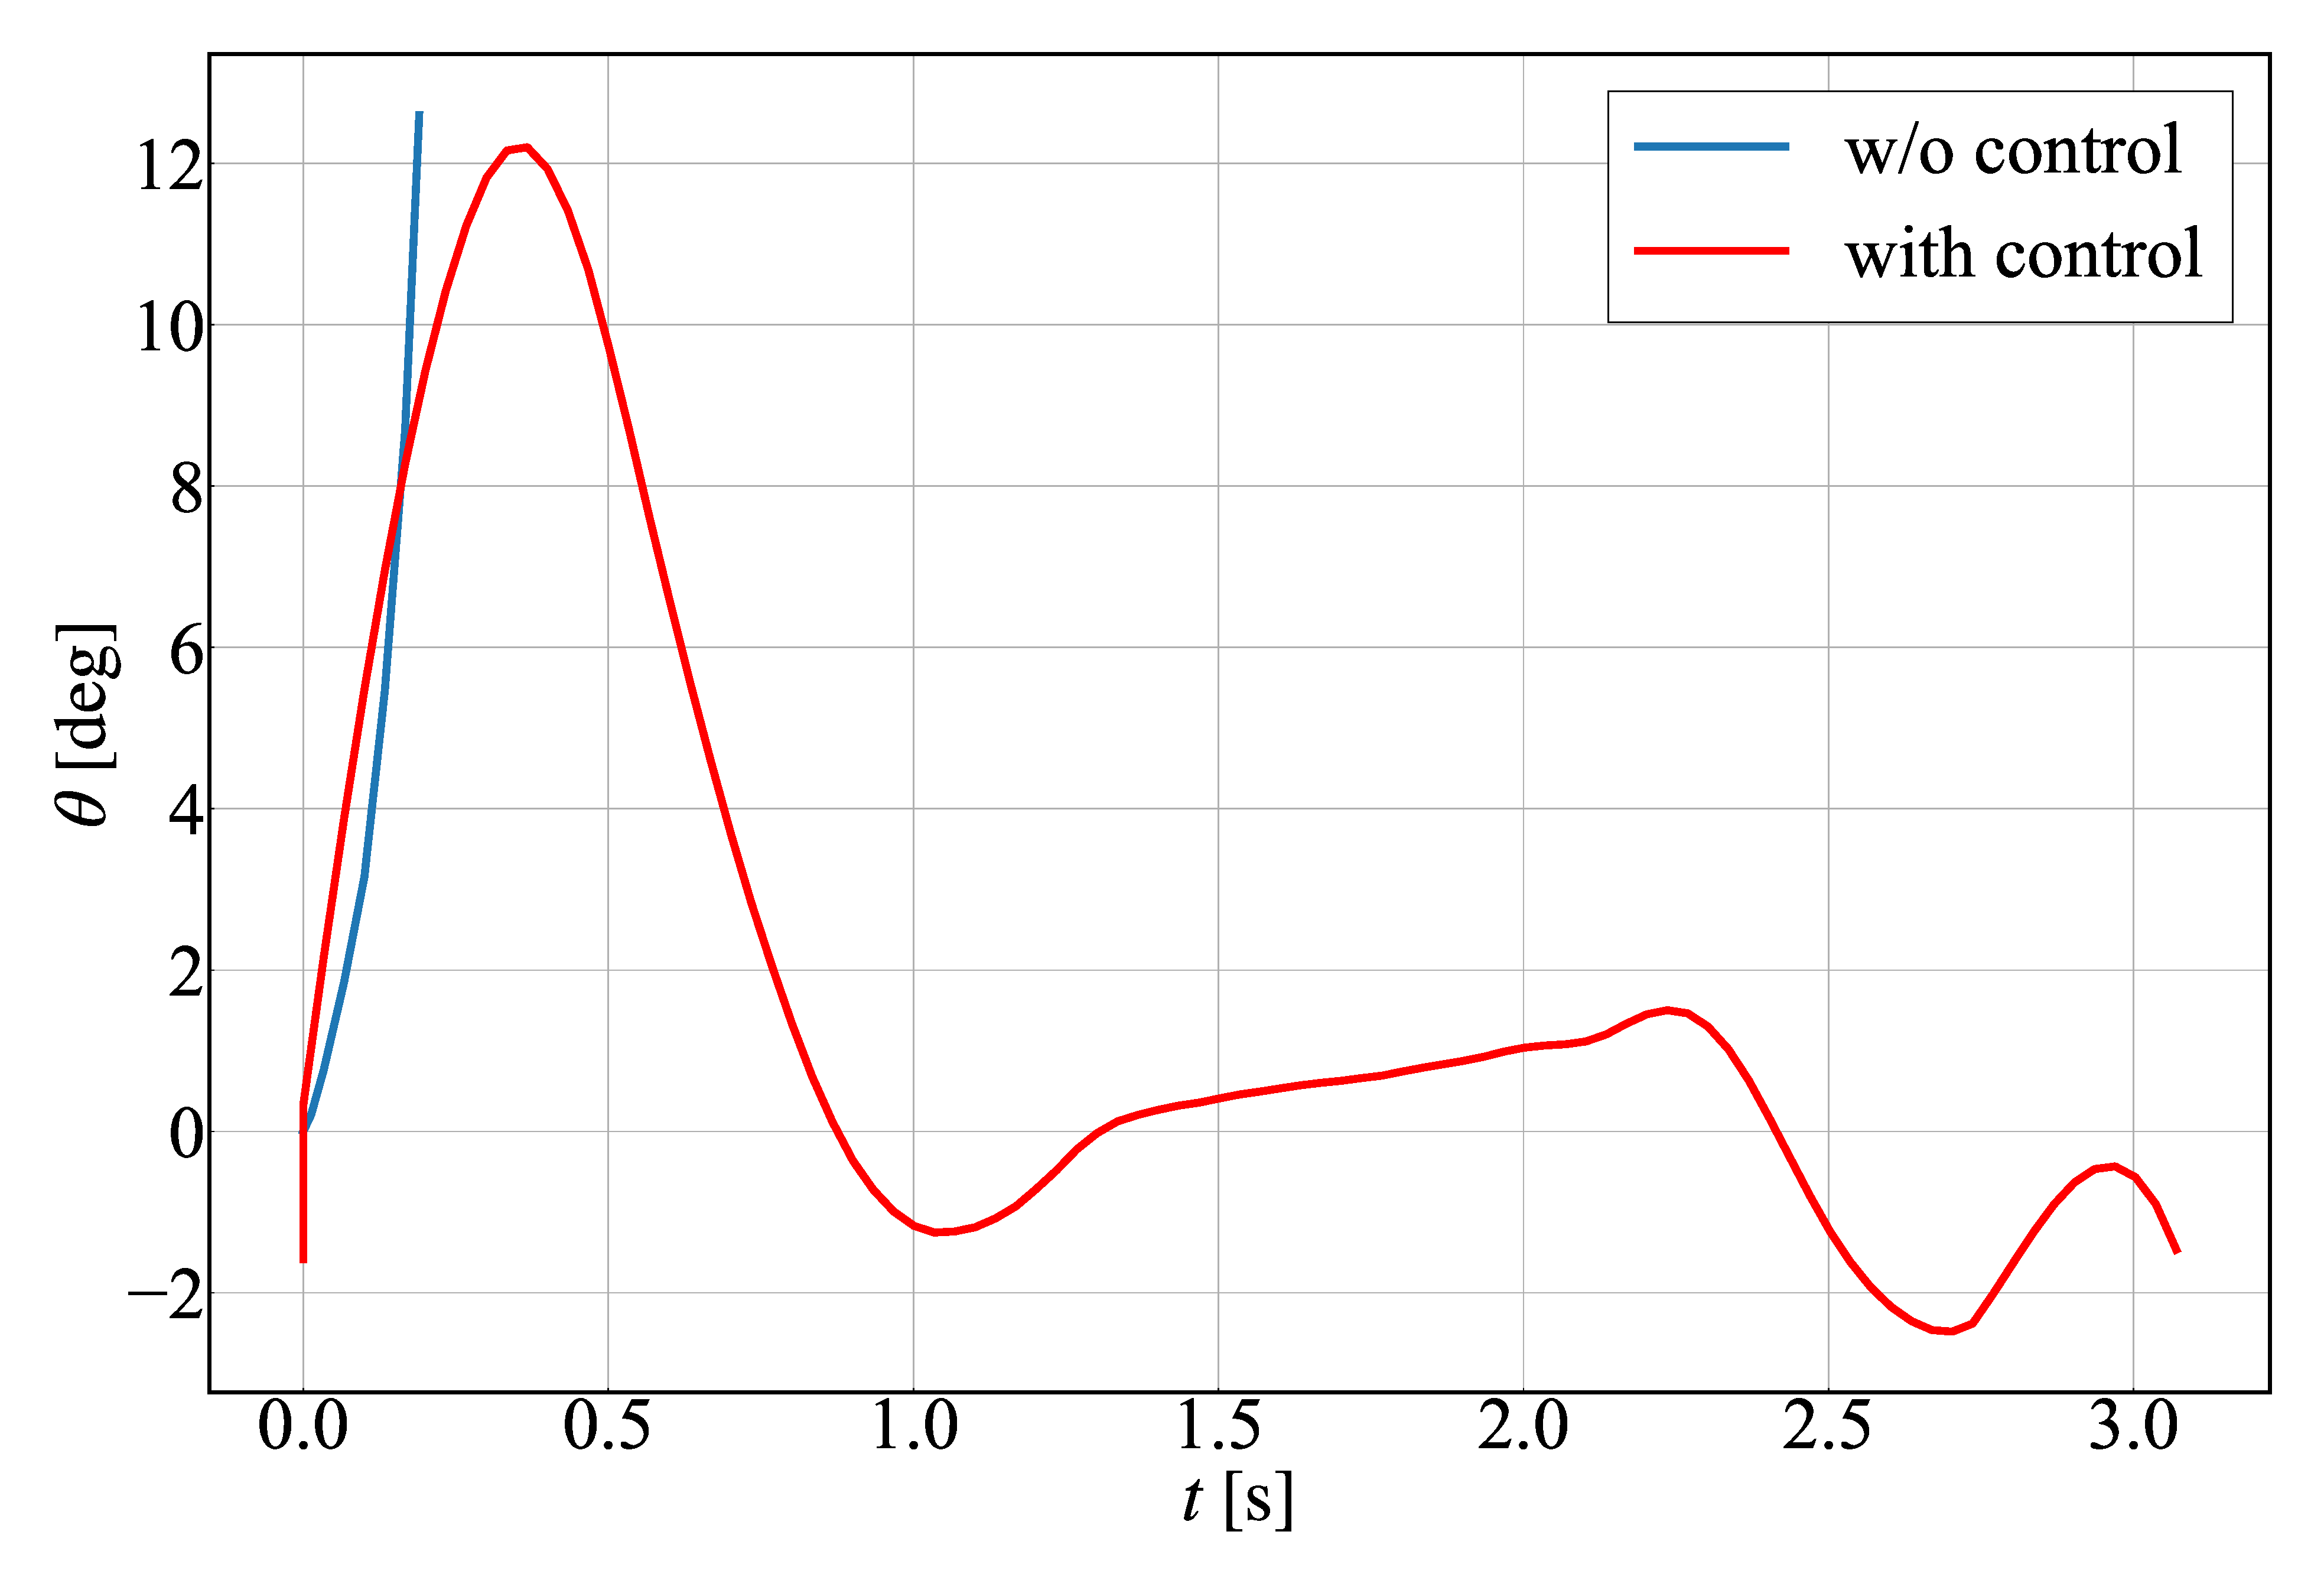
\includegraphics[width=0.6\columnwidth]{figure/angle-control.eps}
     \caption{Change in angle (Control)}
     \labfig{angle-1vC}
   \end{minipage}
  \end{tabular}
\end{figure}
そして,\reffig{acc-1vC}では,横軸は時間,縦軸は紙の動く加速度である.\reffig{acc-1vC}より,牽引装置に電圧を印加する瞬間,つまり時刻が$t=0$~sから$t=0.5$~sの間では制御なしと制御ありの場合両方とも同じ加速度で加速されていることがわかった.牽引装置に同じ電圧を印加し,支持部のロボットの台数も同じなので,加速度が一致していることは妥当である.
また,$t=0.5$~sから$t=2.3$~sの間では加速度は0~\si{m/s^2}付近であるので,等速で移動することが確認できた.その後,牽引装置の印加電圧を遮断すると,全体が減速し,止まることが確認できた.
次に,\reffig{angle-1vC}では,横軸は時間,縦軸は物体の初期姿勢からの角度のずれである.ここで,~\ref{section:exp2}の実験と同じく物体の角度は進行方向の逆向きを正とする.制御なしの場合の角度は設定された$\pm5$\si{\degree}範囲外にあることがわかった.一方,制御ありの場合は,$t=0$~sから$t=0.5$~sまでは,物体の初期姿勢から12\si{\degree}傾いたものの,$t=0.5$~s以降,物体の初期姿勢からの角度差は0に収束し,$\pm1.8$\si{\degree}範囲内に振動することがわかった.
よって,制御をかけることで,ロボット1段でも支持することができると言える.その他,急に動き出すときの大きい角度差に対して,今後ロボットに搭載されている加速度センサを利用して,フィードフォワード制御をかけることで,より安定に運搬できると考えられる.